\chapter{Influence of the solar wind on the oscillations of Jupiter's current sheet}

\section{Introduction}

Ionization of Iogenic neutrals adds  $\sim$1 ton/s of mass to the inner magnetosphere of Jupiter, which increases the content of the corotating flux tubes \cite{Bagenal2011b}. Strong centrifugal forces in the equatorial regions of the Jovian magnetosphere stretch these flux tubes in the radial direction, which leads to the formation of a disk-like current sheet at all longitudes \cite{Khurana2004a} and distorts the magnetic field from the `dipolar' configuration. However, the Jovian current sheet is not static, and its location changes as a function of radial distance and SIII longitude due to various dynamical processes in the magnetosphere. The first such process which modifies the equatorial current sheet was discussed in Chapter 5, where we studied the implications of a thin current sheet which is unstable to the tearing instability. The resulting multiple X-line reconnection creates O-lines and flux ropes on the ion-inertial scale, which can coalesce to form large plasmoids; much like what has been seen at the terrestrial magnetopause and magnetotail \cite{AkhavanTafti2020ComparativeEvents, Eastwood2005ObservationsStudy}.

The second mechanism which perturbs the current sheet is related to the changing planetary magnetic field. Early studies of the Jovian magnetosphere, either through the detection of radio emissions \cite{Carr1969TheJupiter} or in situ spacecraft flybys \cite{Smith1974The10}, had shown that the internal field of the planet could be better described as a dipole which is tilted with respect to the spin axis. The tilted dipole field rotates at the planetary rotation period and introduces a $\sim$10 hour periodicity in the magnetosphere. Magnetic field observations made by Pioneer 10 \cite{Smith1974The10} clearly show this 10-hour periodicity in the form of a `square-wave' signal in the radial component of the magnetic field. These findings were later confirmed by Pioneer 11 \cite{Smith1975Jupiters11}, Voyager 1 and Voyager 2 \cite{Behannon1981}, Galileo \cite{Khurana1992a, Khurana2005} and the Juno spacecraft (see e.g. Figure \ref{fig:juno-current-sheet}). With the introduction of dedicated orbiters, namely Galileo and Juno, more sophisticated models of Jupiter's internal field were developed using spherical harmonics. The VIP4 model was obtained by fitting magnetic field observations from Galileo and uses fourth order harmonics \cite{Connerney1998NewFootprint}, whereas the more recent JRM09 field model \cite{Connerney2018} uses the magnetic field data obtained from Juno's close perijove passes and uses 10th order harmonics. The models show that the Jovian magnetic field is not dipolar and the higher order harmonics have a substantial contribution near the planet. Figure \ref{fig:JRM09} shows the contours of magnetic field magnitude on the 1 bar surface of Jupiter as per the JRM09 magnetic field model. 

Another mechanism which temporarily modifies the structure of the current sheet is in the form of perturbations with frequencies smaller than that of the planet's rotation. One such transient perturbation relates to times when multiple current sheet crossings are observed within an interval of roughly 1 to 2 hours. This phenomena is termed as `magnetotail flapping' and is also seen to occur in the terrestrial and Kronian magnetosphere \cite{Volwerk2013ComparativeSaturn}. Other transient perturbations which occurs on timescales of a few minutes have also been in Saturn's magnetosphere \cite{Martin2017CassiniMagnetodisc}.  

\begin{figure}
    \centering
    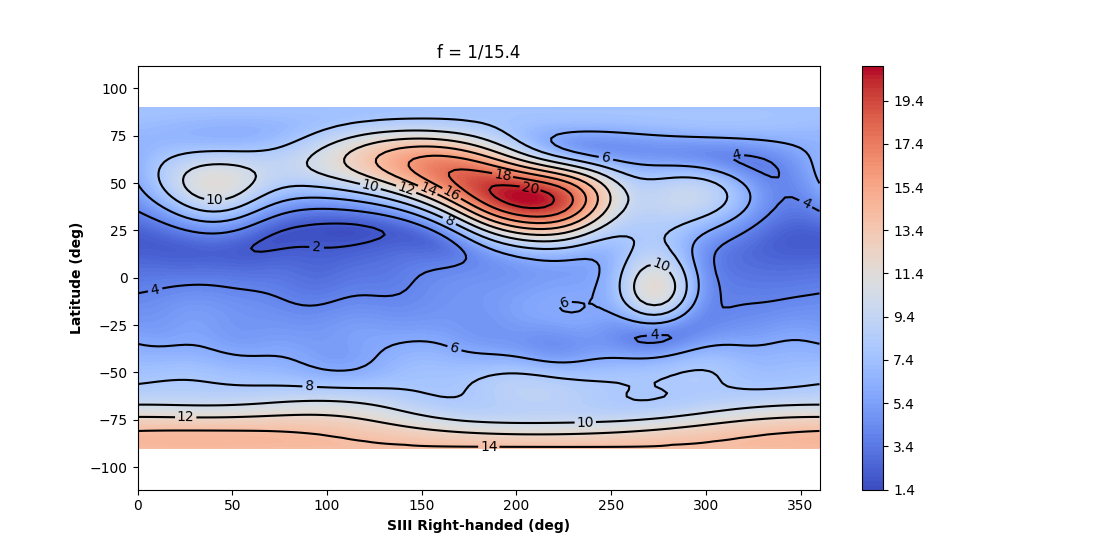
\includegraphics[width=\textwidth]{images5/JRM09_Bmag.png}
    \caption{Contours of the magnetic field strength (in Gauss) on a representative flattened ellipsoid surface of Jupiter as per the JRM09 magnetic field model. The System III longitude system is a left-handed planetocentric coordinate system often used in studies of the Jovian system. In this system, the planetary magnetic field is constant
    \protect\cite{Connerney2018}.}
    \label{fig:JRM09}
\end{figure}

\begin{figure}
    \centering
    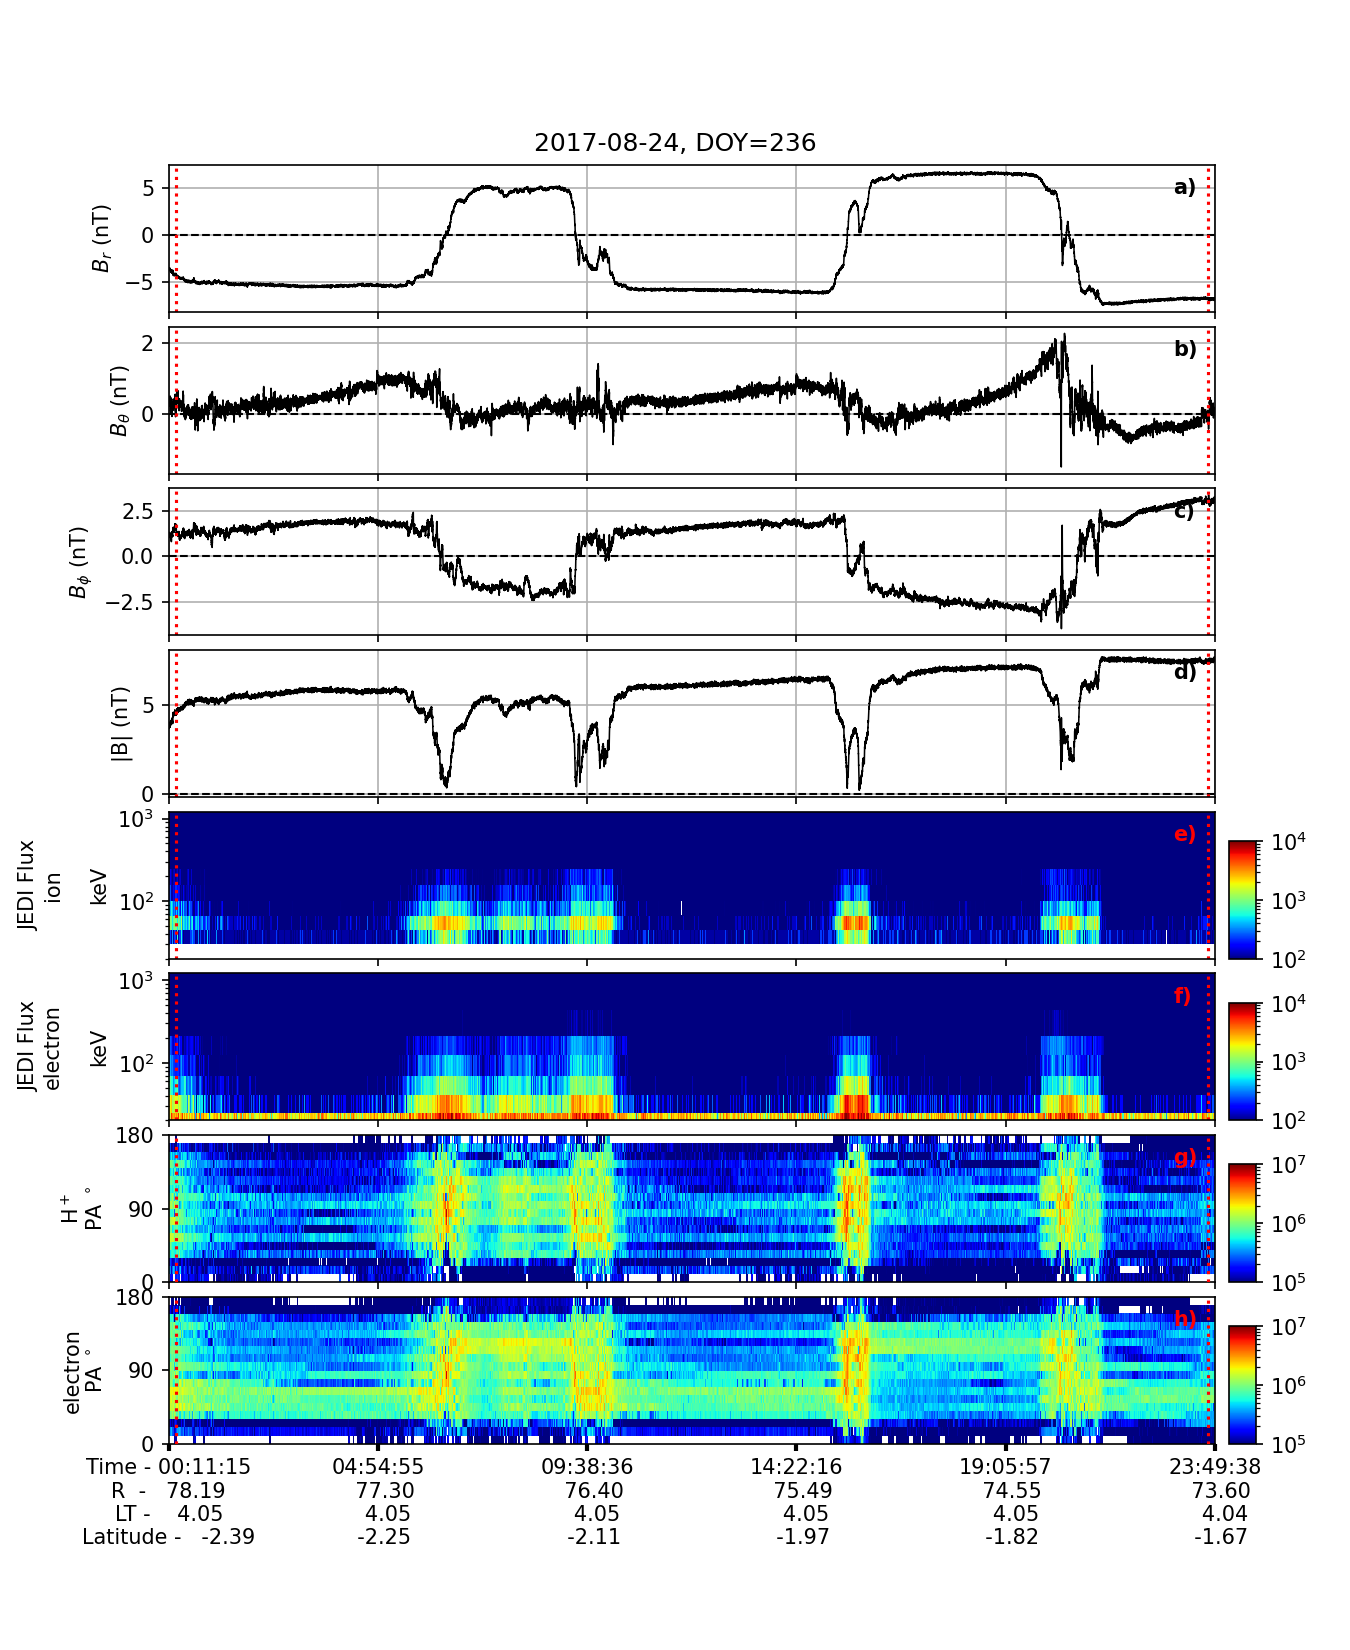
\includegraphics[height=0.8\textheight]{images5/Juno-currentsheet-magjedi.png}
    \caption{Magnetic field and energetic particle (JEDI) measurements taken by the Juno spacecraft in the JSS coordinate system ($B_r$, $B_\theta$, $B_\phi$, $|B|$). Juno crosses the current sheet and plasma sheet twice every rotation period, as seen in the multiple reversals of $B_r$ accompanied with an intensification of particle fluxes separated by roughly $\sim$5 hours. Note the different temporal separation for north-to-south versus south-to-north crossings.}
    \label{fig:juno-current-sheet}
\end{figure}

Many empirical models have been put forward to account for the variation of the Jovian current sheet due to the non-axisymmetric internal field (see e.g \citeNP{Khurana2005} and references therein). Each model has a different set of parameters which are varied to minimize the error between the modeled current sheet location and that seen in situ by the relevant spacecraft. Although they can be used to infer the location of the current sheet, these empirical models do not provide any information about its strength. On th other hand, models have also been develop to estimate the current sheet strength and its contribution to the distortion of the planetary field (e.g. 
They can be categorized into two classes, which are discussed in the later sections. 

 After the flybys of Voyager 1 and 2, it was discovered that the current sheet crossings associated with a North-to-South rotation of the field were delayed compared to those associated with a South-to-North rotation of the field \cite{Behannon1981}. This led to the development of the concept called magnetotail `hinging', which proposed that instead of following the magnetic dipole equator at large radial distances, the maximum  extent of the current sheet was limited to certain heights in the $z$ direction. An example of current sheet hinging is shown in Figure \ref{fig:example-hinging}, where two current sheets are shown with and without the hinging parameter. In a highly hinged current sheet, a spacecraft located above the $z=0$ plane would spend a majority of its time either in the northern lobe or the southern lobe. In Figure \ref{fig:juno-current-sheet}, we show an example of a period when Juno is located predominantly in southern magnetotail lobe (where $B_r<0$), and spends less time in the northern magnetotail lobe ($B_r>0$) due to the hinging of the current sheet. 
 
The current sheet models were modified to include the hinging phenomena, based on heuristic arguments that hinging was a product of Jupiter's magnetospheric interaction with the solar wind and the formation of a magnetotail. \citeA{Behannon1981} showed that the inclusion of current sheet hinging decreased the RMS error between the modeled current sheet and the in situ data, with which it was originally fitted, compared to models which did not include hinging. 
 
In the following sections a description of various empirical models used to fit the in situ observations is provided. 

\subsection{Axial models of the current sheet}
Initial models assumed that the Jovian current sheet would be located in a plane corresponding to the magnetic equator of Jupiter, which would rotate at the planetary rotation period. The expected $z$ location of the current sheet at a given radial location in cylindrical coordinates $(\rho, \phi)$ could then be described simply as \cite{VanAllen1974EnergeticJupiter,Goertz1976TheMagnetosphere},

\begin{equation}
    z = -\rho \tan\theta_d \cos\left(\phi - \phi_d\right)
\end{equation}

Where $\theta_d$ is the tilt of the assumed planetary dipole field with respect to the rotation axis and $\phi_d$ provides the azimuthal location of the magnetic North pole. The rigid tilted plane model was found to be inaccurate at large distances, and the model was modified to limit the $z$ excursions of the current sheet at large radial distances. The first \emph{hinged} current sheet models \cite{Smith1974The10,Hill1974ConfigurationMagnetosphere} added a condition to limit these excursions beyond $\rho > a$, where $a$ was chosen as the hinging distance and was the only free parameter.
\begin{equation}
    z = \begin{cases}
    -\rho \tan\theta_d \cos\left(\phi - \phi_d\right), & \text{for } \rho \leq a\\
    -a \tan\theta_d \cos\left(\phi - \phi_d\right), & \text{for } \rho > a
    \end{cases}
\end{equation}

Or alternatively, using a $\tanh$ function, 
\begin{equation}
    z = -a \tanh\left(\frac{\rho}{a}\right) \tan\theta_d \cos\left(\phi - \phi_d\right)
\end{equation}

An improvement was suggested by \citeA{Kivelson1978ASheet} in the form of a phase delay to the current sheet location, proportional to the distance from the wave source and had the following functional form,
\begin{equation}
    \phi' = \phi_d - \frac{\Omega \left( \rho - \rho_0\right)}{U}
\end{equation}

Where $\Omega$ was the angular velocity of Jupiter, $U$ was the speed at which the wave travelled and $\rho_0$ served as the radial distance where the current sheet ceased to follow the rotating plane, beyond which all locations perceived a delay in the arrival of the current sheet. The expected current sheet location in the \citeA{Kivelson1978ASheet} model was then given by,
\begin{equation}
    z = \begin{cases}
    -\rho \tan\theta_d \cos\left(\phi - \phi_d\right), & \text{for } \rho < \rho_0\\
    -\rho \tan\theta_d \cos\left(\phi - \phi'\right),  & \text{for } \rho \geq \rho_0
    \end{cases}
    \label{eqn:kivelson1978}
\end{equation}

\citeA{Eviatar1976PlasmaMagnetosphere} introduced a similar model but limited the latitudinal extent of the oscillation beyond $\rho \geq \rho_0$,
\begin{equation}
    z = \begin{cases}
    -\rho \tan\theta_d \cos\left(\phi - \phi_d\right), & \text{for } \rho < \rho_0\\
    -a \tan\theta_d \cos\left(\phi - \phi'\right),  & \text{for } \rho \geq \rho_0
    \end{cases}
\end{equation}

Lastly, \citeA{Behannon1981} introduced another axial model which included the effects of wave propagation and current sheet hinging (Equation 11 in \citeA{Behannon1981}). However, they assumed that the wave starts propagating from the origin i.e. $\rho_0=0$.
\begin{equation}
    z = -a \tanh\left(\frac{\rho}{a}\right) \tan\theta_d \cos\left(\phi - \phi_d + \frac{\Omega \rho}{U}\right)
    \label{eqn:behannon1981}
\end{equation}

\subsection{Non-axial models of the current sheet}
Axial models were found to fit the data poorly at large distances in the magnetotail, and it was suggested that the interaction of the magnetosphere with the solar wind may lead to a formation of a magnetotail, where the current sheet would take the form of a rocking plane instead of a rotating disk. However, the rocking plane model did not accurately represent the current sheet near the planet. \citeA{Behannon1981} suggested a hybrid model which followed the magnetic equator close to the planet and took the form of a rocking plane at large distances (also called the Rocking Plane/Rotating Disk model or RP/RD).

\begin{equation}
    \phi' = \phi_d - \frac{\Omega \left(x - a\right)}{U}
\end{equation}
\begin{equation}
    z = x \sech \left( \frac{x}{a} \right) \cos\left(\phi - \phi' \right) + y \sin\left(\phi - \phi' \right)  
\end{equation}

Note that the above model follows a rotating disk near the planet where $\phi'=\phi_d$. The wave starts propagating at distance $a$ at a fixed speed $U$, which are the two parameters for this model. \citeA{Khurana1992a} extend the previous models by prescribing a variation in the wave propagation speed with radial distance as follows,

\begin{equation}
    v(\rho) = v_0 \coth \left(\frac{\rho}{\rho_0} \right)
\end{equation}
which leads to the following expressions for the phase delay and the current sheet location,
\begin{equation}
    \phi' = \phi_d - \Omega \int \frac{d\rho}{v(\rho)} = \phi_d - \frac{\Omega \rho}{v_0} \ln \cosh \left( \frac{\rho}{\rho_0} \right) 
\end{equation}
\begin{equation}
    z = -\rho \tan\theta_d \cdot \frac{x_0}{x} \tanh\left(\frac{x}{x_0} \right) \cos\left( \phi - \phi'\right) 
    \label{eqn:khurana1992}
\end{equation}
The \citeA{Khurana1992a} model had three parameters $(v_0, \rho_0, x_0)$ representing the asymptotic wave propagation speed, radial location of outflow, and the hinging point along the X-axis to account for the interaction with the solar wind. \citeA{Khurana2005} updated the model to account for local time asymmetries and solar wind angle of attack, but the generalization increased the number of parameters in the model. 

\begin{figure}
    \centering
    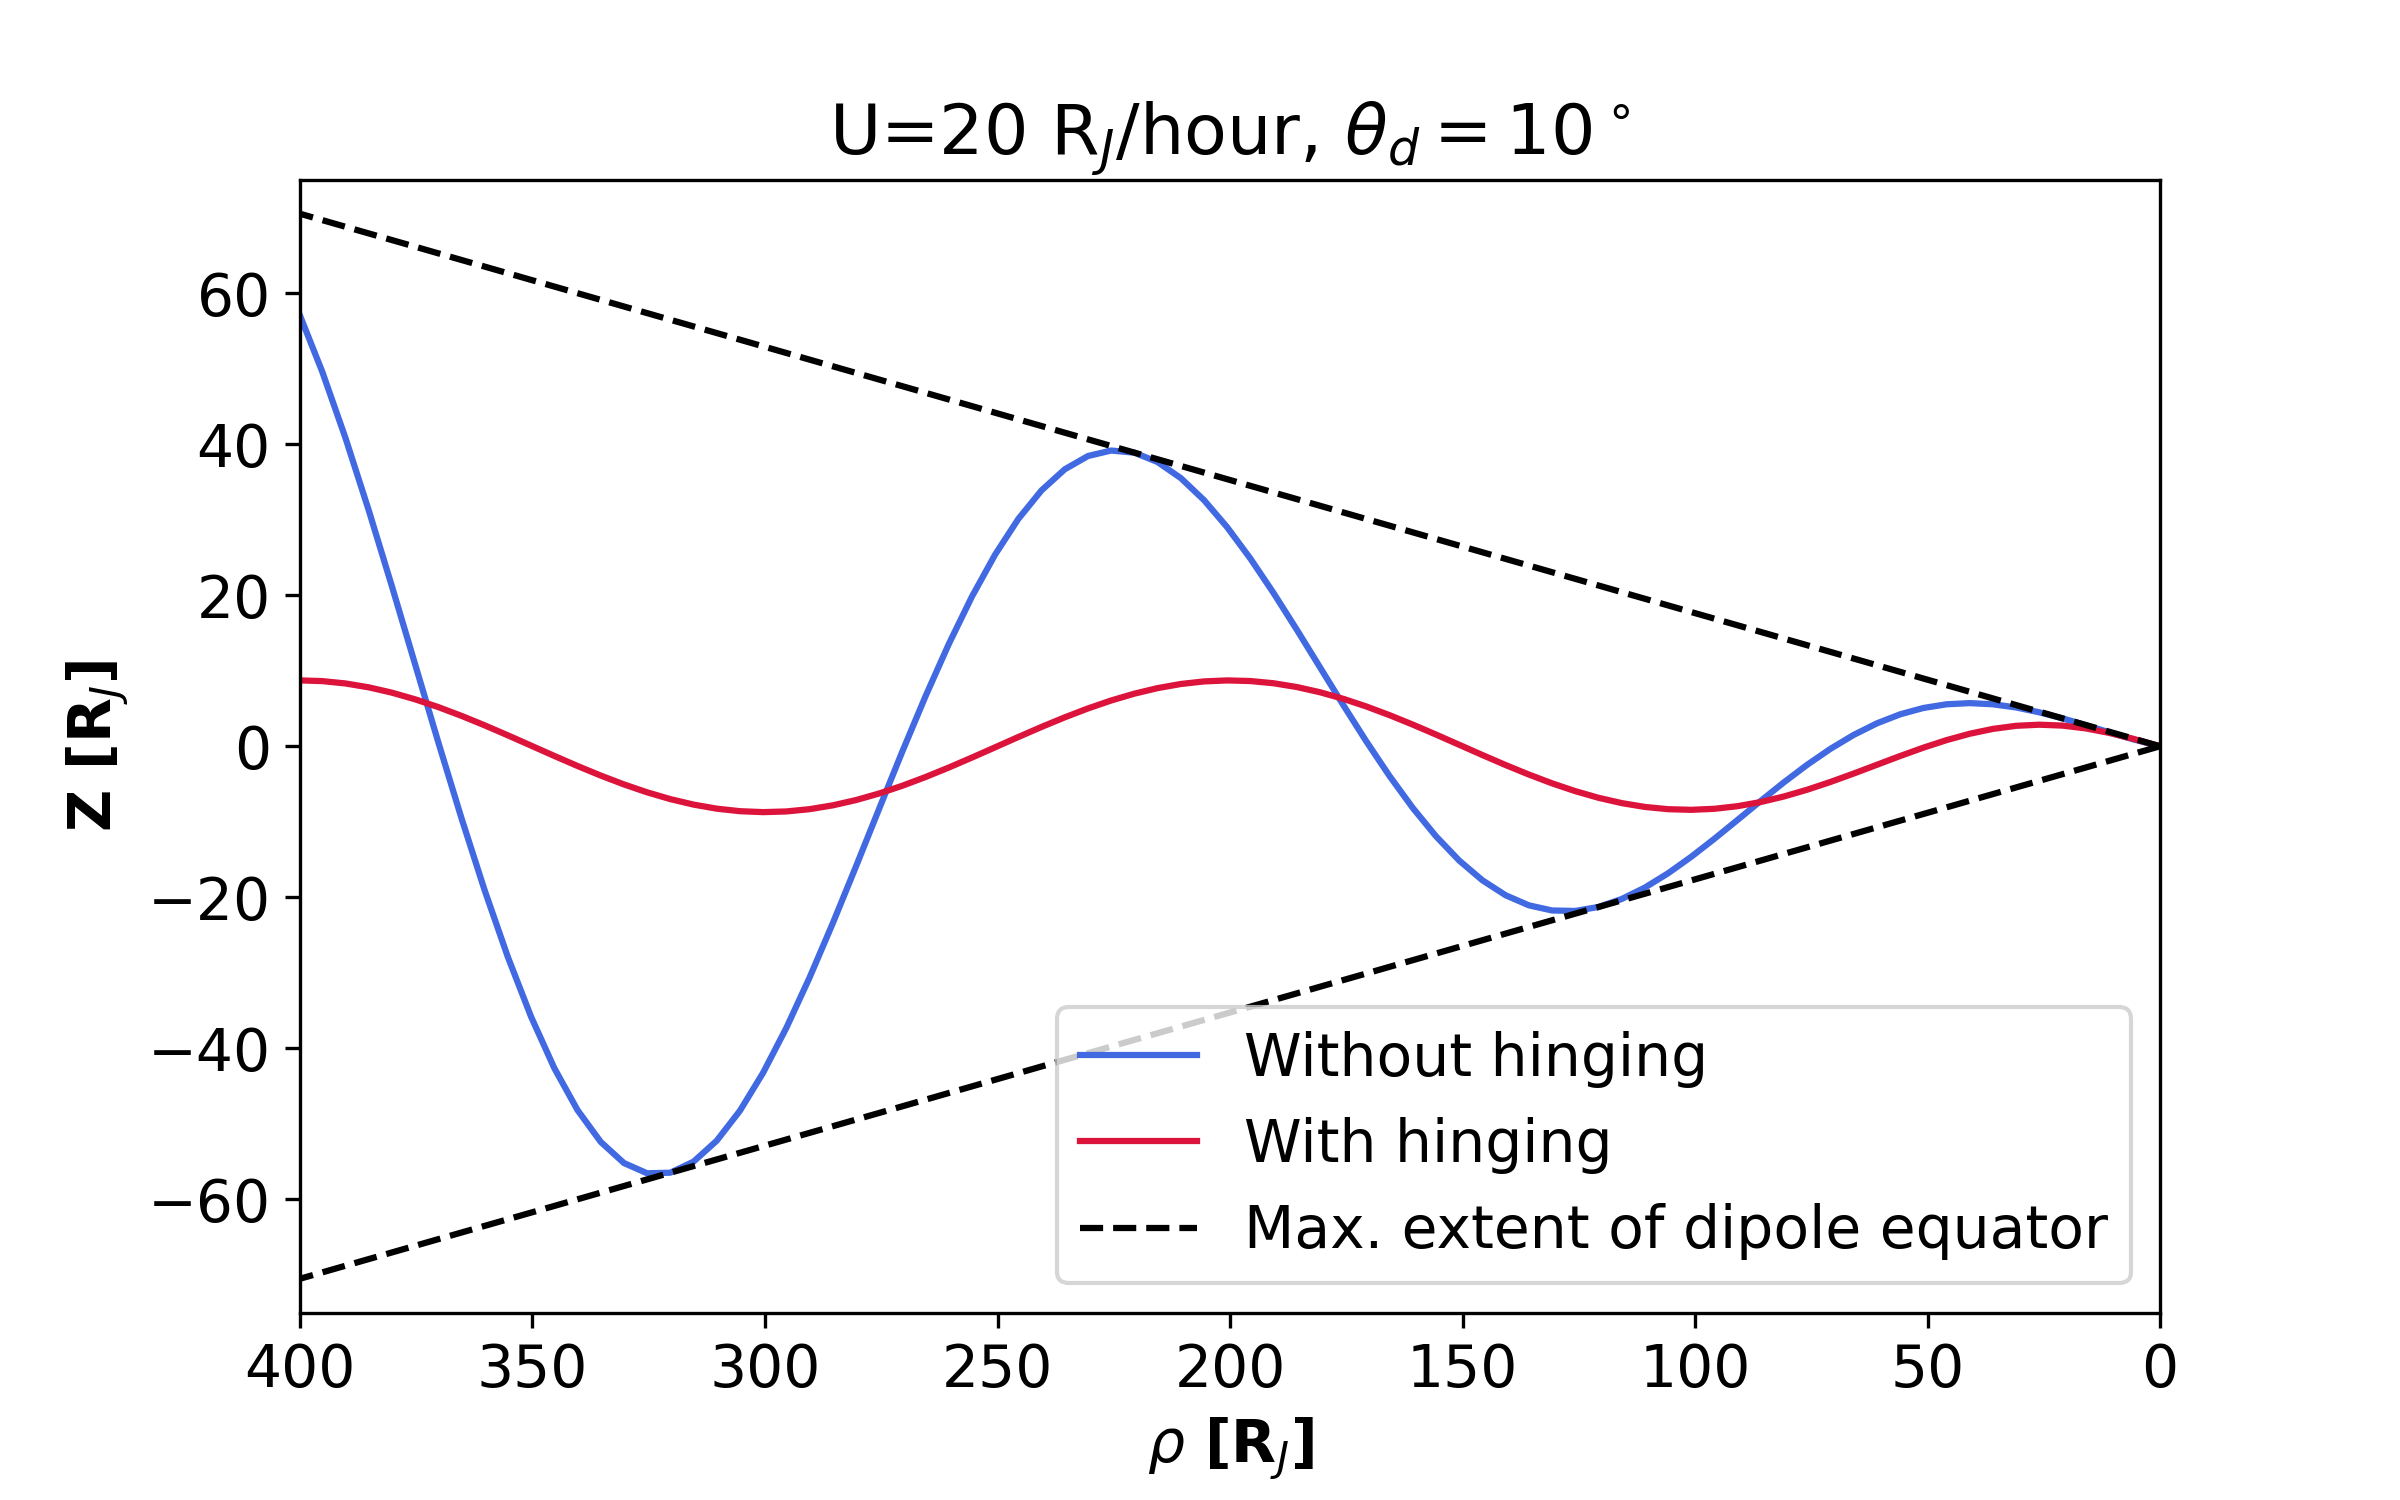
\includegraphics[width=0.8\textwidth]{images5/example-hinging.png}
    \caption{Exaggerated examples of the Jovian current sheet locations for two different models. The \protect\citeA{Kivelson1978ASheet} model does not account for hinging of the current sheet and hence has larger excursions with increasing distance from the planet. The \protect\citeA{Behannon1981} model includes current sheet hinging, which limits the oscillations beyond a certain radial distance.}
    \label{fig:example-hinging}
\end{figure}

\subsection{Objective of this study}

In Chapters 4 and 5 we showed that the Jovian magnetosphere, which was previously assumed to be insensitive to changes in the upstream parameters, does respond to changes in the solar wind dynamic pressure and the interplanetary magnetic field in the form of changes to the magnetospheric configuration and strength of currents in the ionosphere. In this chapter, we discuss the influence of the solar wind dynamic pressure on the Jovian current sheet. Specifically, we seek to answer the following questions,

\begin{itemize}
    % \singlespacing
    \item Does solar wind dynamic pressure increase or decrease the hinging distance of the current sheet?
    \item Does solar wind dynamic pressure change the speed at which the current sheet wave propagates outward from the planet?
    \item What are the differences in the response of a magnetosphere to a forward shock in the solar wind when using an idealized versus a tilted dipole for the internal field?
\end{itemize}


\section{Methodology}

\subsection{MHD simulations with a tilted dipole}
To simulate the modulation of the Jovian current sheet, we modify the internal magnetic field of Jupiter to take the form of a dipole which is tilted 10$^\circ$ with respect to the spin axis and which rotates around it at the planetary rotation period (10 hours). The simulations are performed in the GSE coordinate system, where the rotation is enforced about the $z$ axis. In this system, the magnetic poles of the planet trace a circular path around the geographic pole. 

In the simulations shown in Chapters 3 and 4, we used a spherical grid. Through our tests, we found that a spherical grid is not ideal when simulating a time-varying magnetosphere, where density and magnetic structures frequently cross the polar regions of the planet where grid cells are small and have a large aspect ratio for a spherical grid. To prevent this problem, we use a cartesian grid in the simulations performed for the present study. Like the previous version, we use the capability of the BATSRUS MHD code to successively refine regions of interest, such as the Io torus and the low-latitude middle and outer magnetosphere where the current sheets oscillations take place. The cartesian grid contains roughly 19 million cells, with the lowest grid resolution of 0.125 $R_J$ present near the planet and the Io torus. 

Different upstream conditions are introduced to evaluate the response of the current sheet to varying solar wind dynamic pressure. The properties of the solar wind used for the three runs are tabulated in Table \ref{tab:sw-conditions-chp5}. The solar wind dynamic pressure increases by a factor of 5 between each run. 

\begin{table}
    \centering
    \begin{tabular}{c|c|c|c|c|c}

    Run  &$B$  &$u$  &$\rho$     &$T$  &$p_d=\rho u^2$\\
         &nT   &km/s &amu/cm$^3$ &K    &nPa\\
    \hline
    1    &0.31  &322.04  &0.062  &4.3E2  &0.011\\
    2    &1.00  &400.00  &0.200  &2.0E5  &0.053\\
    3    &2.82  &532.46  &0.564  &8.8E5  &0.267\\

    \end{tabular}
    \caption{Solar wind magnetic field strength, speed, density, temperature and dynamic pressure used in the present study. The variables are prescribed at the upstream boundary of the simulation at $X=192$ $R_J$. The interplanetary magnetic field is oriented along the negative $Z$ direction.}
    \label{tab:sw-conditions-chp5}
\end{table}

\subsection{Estimating the current sheet parameters within the MHD model}
The current sheet can be identified as the locus of points in the closed magnetosphere region where $B_r=0$. Its location in our model varies with radial distance and dipole phase. A direct comparison between the current sheet location in the MHD model and the various empirical functions shows a poor fit, as small differences in phase can lead to large differences in the final current sheet location. Moreover, the empirical models have been observed to perform well only for the in situ data to which they were originally fitted \cite{Khurana1992a, Behannon1981}. For a more accurate comparison, we use the functional form for the various empirical models to find the set of parameters e.g. hinging distance, wave propagation speed, etc. which reproduce best the output seen in the MHD simulations. Then, we compare the parameters obtained by fitting the in situ data, to those obtained by fitting the MHD simulation results. 

We consider three models with relatively simple functional forms,
\begin{enumerate}
    \item The \citeA{Kivelson1978ASheet} model described by Equation \ref{eqn:kivelson1978} with two parameters - $U$ and $\rho_0$, corresponding to the speed of wave propagation and the radial location where the current sheet wave starts to propagate. 
    \item The \citeA{Behannon1981} model described by Equation \ref{eqn:behannon1981} with two parameters - $U$ and $a_0$, corresponding to the speed of wave propagation and the radial location where hinging is introduced.
    \item The \citeA{Khurana1992a} model described by Equation \ref{eqn:khurana1992} with three parameters - $v_0$, $x_0$ and $\rho_0$, corresponding to the asymptotic speed of wave propagation, the characteristic hinging distance in the $x$ direction and the radial location where the wave outflow commences. 
\end{enumerate}

The location of the current sheet is extracted in the noon-midnight meridian (00 LT) by identifying the locus of points located between $x=[-100, -4] R_J$ and $z=[-30, 30] R_J$ where  $B_r=0$. A current sheet model is then fitted to the extracted current sheet height $z_\text{MHD}$ at a given radial location $\rho$ by finding the set of parameters $\boldsymbol\theta$ that minimizes the square of the residual $\mathcal{R}$, which is normalized to the standard deviation of the current sheet location in the MHD model ($z_\text{MHD}$),

\begin{equation}
    \mathcal{R} = \frac{1}{\sigma(z_\text{MHD})} \sum_i^N \left[ z_\text{MHD}(\rho) - z_\text{fit} (\rho, \boldsymbol\theta) \right]_i^2
\end{equation}

The Levenberg-Marquardt iterative algorithm \cite{Newville2018Non-LinearPython,Levenberg1944ASquares} is used to perform the non-linear minimization for all models. We repeat the above procedure for all simulation data files separated by an interval of 30 minutes, giving us 200 data points within a 100 hour interval for each model. Although we limit our analysis to regions in the $y=0$ plane and for $x < -4 R_J$ (i.e., the nightside magnetotail), we effectively sample different phases of the current sheet due to the rotation of the dipole every 10 hours. Times when a good fit to the MHD output cannot be obtained are identified by evaluating the magnitude of model uncertainties and comparing them to the parameter values, and are subsequently discarded. 

\begin{figure}
    \centering
    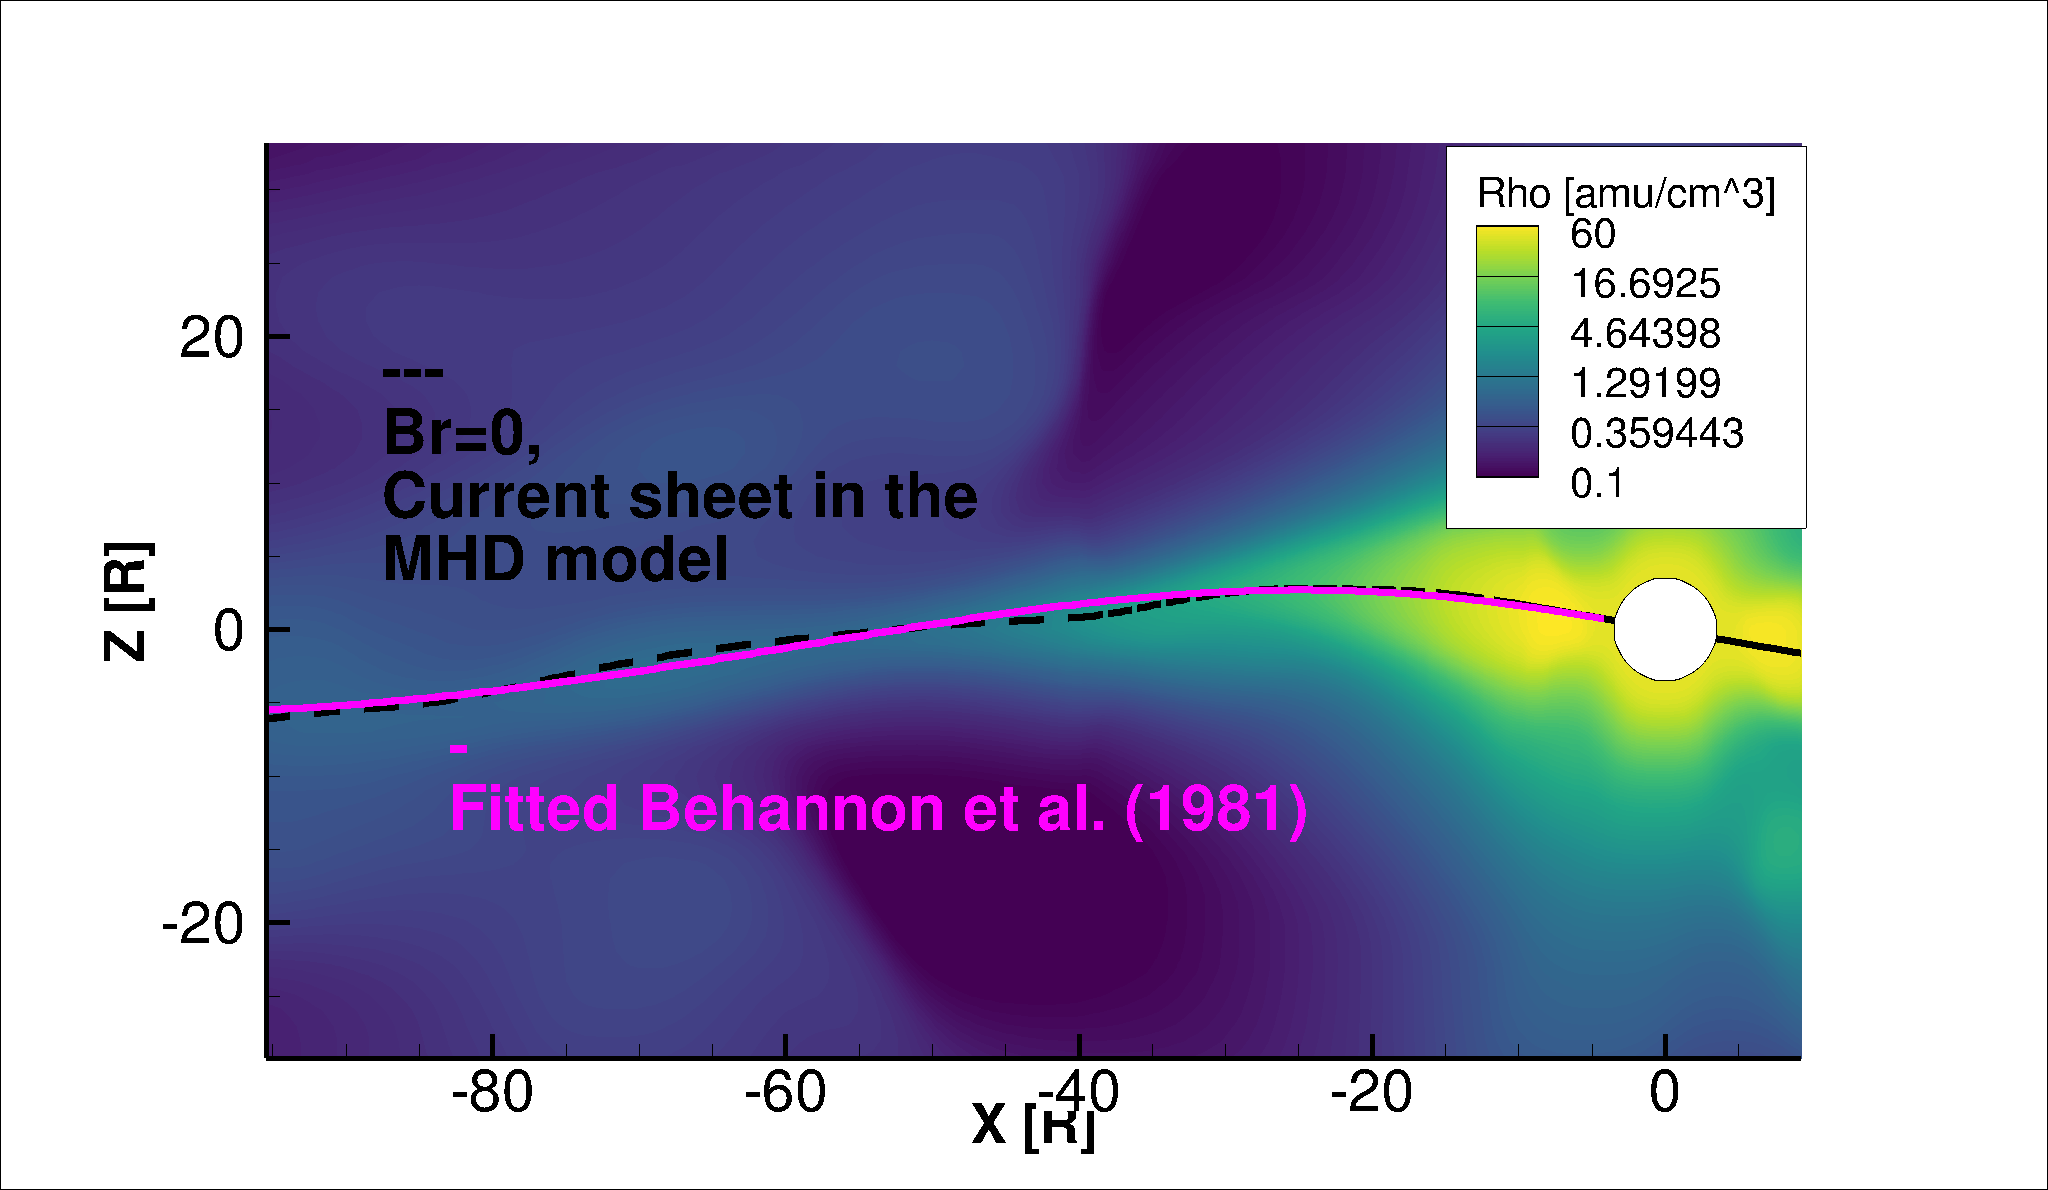
\includegraphics[width=\textwidth]{images5/CurrentSheet_fitted.png}
    \caption{An example of the current sheet extracted from the MHD model  by identified the contour line where $B_r=0$ (dashed black curve), along with the fitted current sheet using the Behannon et al. (1981) form (magenta).}
    \label{fig:example-fitcurrentsheet}
\end{figure}

Figure \ref{fig:example-fitcurrentsheet} shows the result of fitting the \citeA{Behannon1981} model for the current sheet to that observed at that instance in the MHD simulations. In this instance, the wave velocity $U$ and the hinging distance $a_0$ are estimated to be 20.8 $R_J$/hour (413.0 km/s) and 32.4 $R_J$ respectively. 

\section{Results}

We investigate the response of the current sheet parameters to the solar wind dynamic pressure by introducing three different upstream cases which are described in Table 1. 

\subsection{The Kivelson et al. (1978) form}

\begin{figure}
    \centering
    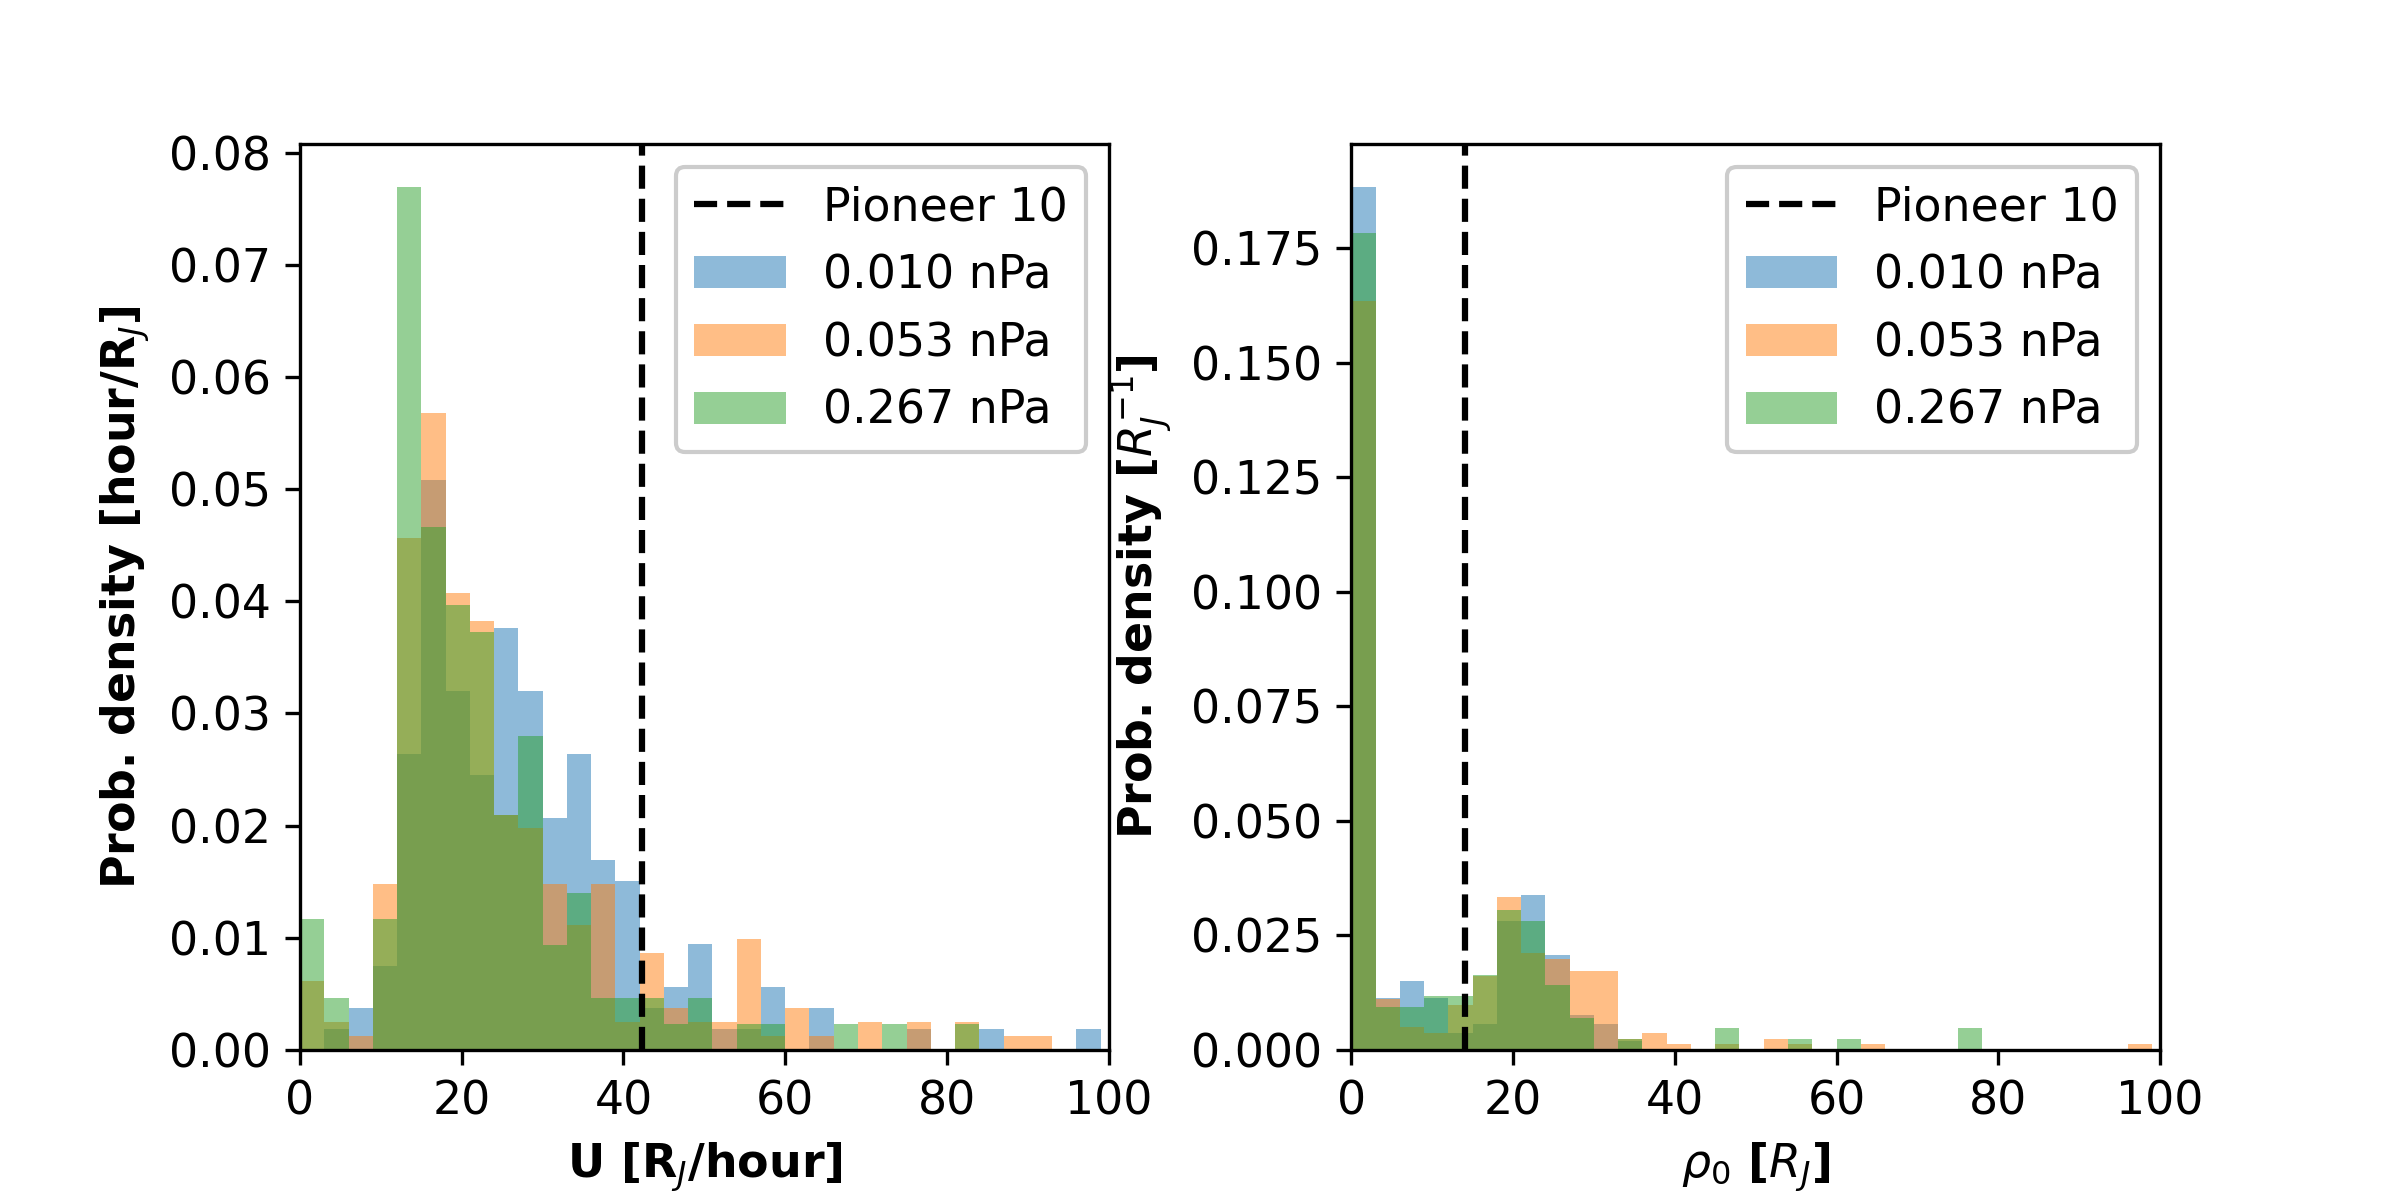
\includegraphics[width=\textwidth]{images5/comparison_highdynP_kivelson.png}
    \caption{Histograms of the parameters used to fit the Kivelson et al. (1978) model form to the current sheet in the MHD model. Different colors represent the different solar wind dynamic pressures.}
    \label{fig:comparison-hist-kivelson}
\end{figure}

\begin{table}
    \centering
    \begin{tabular}{c|c|c|c|c|c}
     $p_\text{dyn}$&      $N$&     mean$(U)$ &   $\text{median}(U)$ &  mean$(\rho_0)$ &   $\text{median}(\rho_0)$\\
     nPa&  &  $R_J/$hour& $R_J/$hour& $R_J$& $R_J$\\
    \hline
     0.010 &  177 &  28.06 &  25.83 &   8.14 &     0.00 \\
     0.053 &  270 &  25.57 &  20.94 &  12.15 &     3.74\\
     0.267 &  143 &  22.17 &  18.93 &  10.88 &     0.00 \\

    \end{tabular}
    \caption{Statistics of the fits to the Kivelson et al. (1978) model shown in the histograms in Figure \protect\ref{fig:comparison-hist-kivelson}. $N$ is the total number of good fits in each case.}
    \label{tab:comparison-kivelson}
\end{table}


Fitting Equation \ref{eqn:kivelson1978} to the current sheet extracted from the simulation yield two parameters - the wave propagation speed $U$ and the radial location where wave propagation begins $\rho_0$. The parameters which fit best the simulation results are plotted in a histogram in Figure 
\ref{fig:comparison-hist-kivelson} for the three dynamic pressures and their properties are shown in Table \ref{tab:comparison-kivelson}. The number of simulation times for which a good fit is obtained varies between the different runs. For a meaningful comparison, we show the probability density instead of the total number of events in each bin (i.e. in our case the area under each histogram sums to unity). 

The histograms for the wave propagation speed show a range of possible values, from $\sim$10 $R_J$/hour (198.6 km/s) to $\sim60 R_J$/hour (1191.5 km/s), though the distribution is skewed to lower values. With increasing dynamic pressure, the distribution shifts more to lower values, indicating that the wave propagation speed is lower during intervals when the solar wind dynamic pressure is high. This can also be seen in Table \ref{tab:comparison-kivelson}, where higher solar wind dynamic pressure is seen to decrease the mean and median value of $U$, from $\sim28.06$ $R_J$/hour (557.24 km/s) to $\sim22.17$ $R_J$/hour (440.27 km/s). Also shown in Figure \ref{fig:comparison-hist-kivelson} is the $U$ value obtained by \citeA{Kivelson1978ASheet} by fitting the Pioneer 10 data, which is 42.29 $R_J$/hour or 840 km/s. The velocity in our simulations is roughly a factor of 2 less than these results, which could be due to different magnetospheric or external conditions. 

On the other hand, the distribution of $\rho_0$ in the MHD model overwhelmingly favours low values and is insensitive to change in the solar wind dynamic pressure. Low $\rho_0$ values imply that the current sheet wave begins propagating at a finite speed very close to the planet. The mean and median values of $\rho_0$ as shown in table \ref{tab:comparison-kivelson} are $\sim10$ $R_J$ and $\sim 0$ $R_J$ respectively, indicating that although there are some outliers, majority of the fits for low and high solar wind dynamic pressure favour near-zero values for $\rho_0$. A moderate increase is seen for the intermediate case of 0.05 nPa, where the mean and median values increase to $12.74$ $R_J$ and $3.74$ $R_J$ respectively. Although our model predominantly favours near-zero values of $\rho_0$, all histograms show a small peak near $20R_J$. In comparison, the Pioneer 10 observations (shown in black dashed lines in Figure \ref{eqn:kivelson1978}) estimate this outflow to begin from a distance of $\sim14$ $R_J$ \cite{Kivelson1978ASheet}.  

\subsection{The Behannon et al. (1981) form}
\begin{figure}
    \centering
    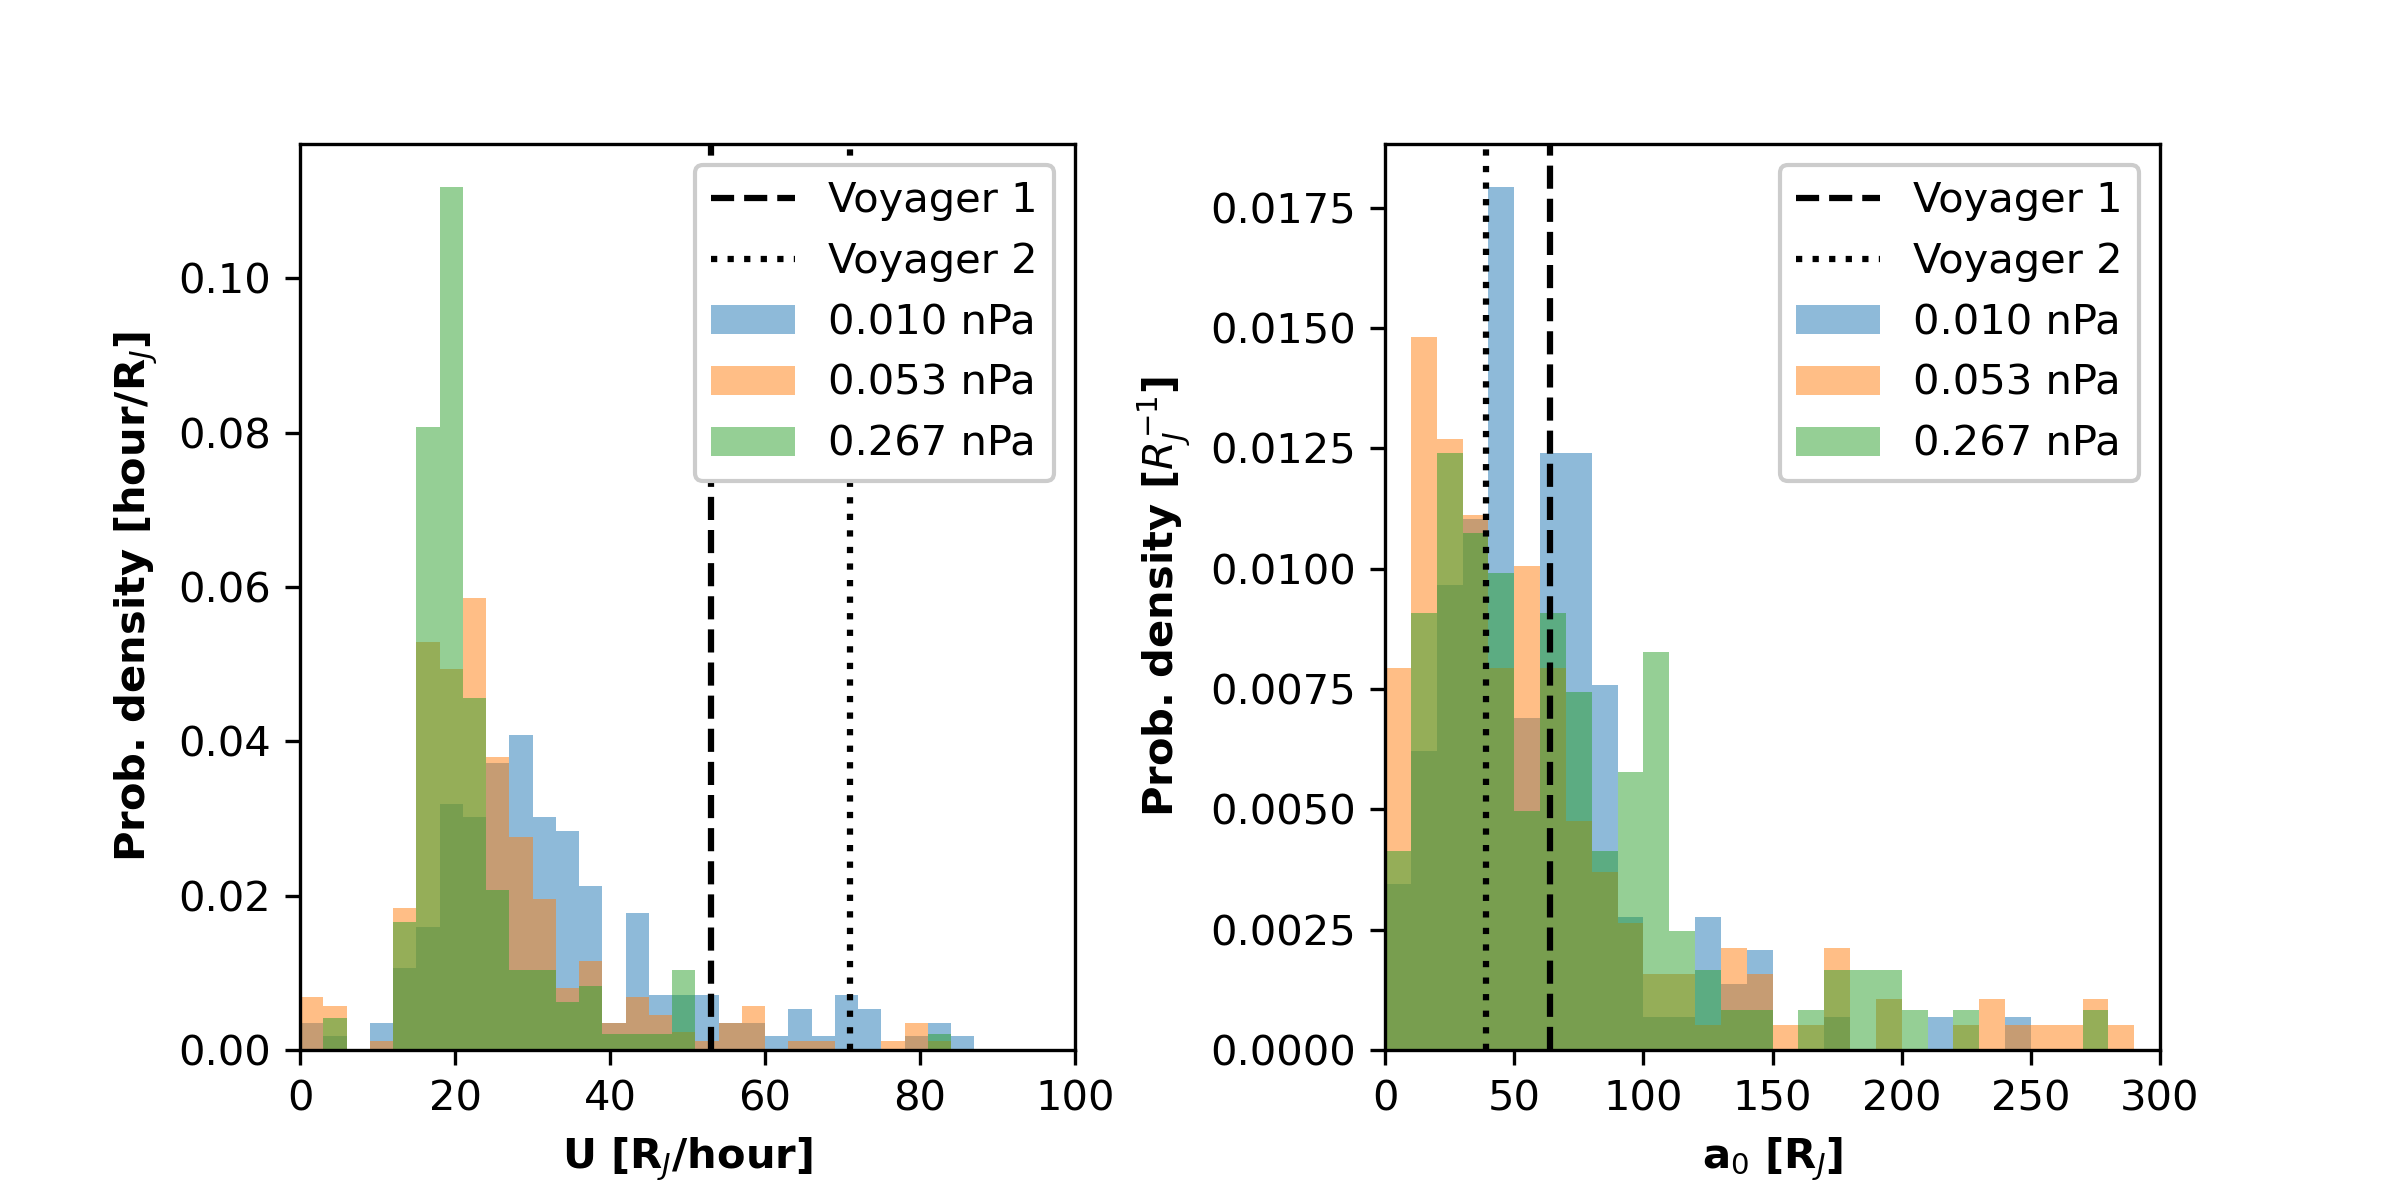
\includegraphics[width=\textwidth]{images5/comparison_highdynP_behannon.png}
    \caption{Histograms of the parameters used to fit the Behannon et al. (1981) model form to the current sheet in the MHD model. Different colors represent the different solar wind dynamic pressures.}
    \label{fig:comparison-hist-behannon}
\end{figure}

\begin{table}
    \centering
    \begin{tabular}{c|c|c|c|c|c}
     $p_\text{dyn}$ &      $N$&  mean$(U)$&  median$(U)$&  mean$(a_0)$&  median$(a_0)$\\
     nPa&   &   $R_J/$hour& $R_J/$hour& $R_J$& $R_J$\\
     \hline
     0.01 & 188 &   33.04 &     29.41 &  2410.45 &      68.67 \\
     0.05 & 290 &   25.45 &     22.28 &  3411.81 &      78.19 \\
     0.27 & 161 &   22.22 &     19.62 &  1986.96 &      75.19 \\
    \end{tabular}
    \caption{Statistics of the fits to the Behannon et al. (1981) model shown in the histograms in Figure \protect\ref{fig:comparison-hist-behannon}. $N$ is the total number of good fits in each case.}
    \label{tab:comparison-behannon}
\end{table}

This model described by Equation \ref{eqn:behannon1981} contains two parameters - the wave propagation speed $U$ and the distance $a_0$ beyond which the current sheet is \emph{hinged}, i.e. the radial location beyond which its maximum extent in the $z$ direction is limited. As before, we show the normalized histograms of these parameters in Figure \ref{fig:comparison-hist-behannon}. 

Similar to the result obtained when using the \citeA{Kivelson1978ASheet} form, the speed of the current sheet wave varies between 15 to 50 $R_J$/hour. For lower solar wind dynamic pressure (0.010 nPa), the mean of the distribution is located at 33.04 $R_J$/hour (656.13 km/s) and shift to lower values for higher solar wind dynamic pressure to 22.22 $R_J$/hour (441.26 km/s). The median values of $U$ also decrease with increasing solar wind dynamic pressure from $29.41$ to $19.62$ $R_J$/hour. Histograms for $U$ for the three different cases clearly show the shift to lower values as the dynamic pressure of the solar wind is increased (Figure \ref{fig:comparison-hist-behannon}). For comparison, the fits from the Voyager 1 and 2 flybys estimate the wave speed to be 53 and 71 $R_J$/hour (or 1052.52 and 1409.98 km/s) respectively, which is roughly 2 to 3 times the values obtained from our simulations. Note that the previous study by \citeA{Kivelson1978ASheet}, which used data from the the Pioneer 10 flyby estimated $U$ to be roughly 840 km/s, which is lower than the Voyager results. 

The hinging parameter $a_0$ also exhibits large variations, with most values ranging between 0 to 100 $R_J$, although there are some outliers with values $>1000 R_J$. In this case, large values of $a_0$ would indicate that the current sheet hinges at large radial distances. There is a large discrepancy between the mean and median values, the former ranging between 1986.96 $R_J$ to 3411.81 $R_J$ and the latter ranging between $68.67 R_J$ to $78.19 R_J$ for the three runs. Large values of $a_0$ are not unrealistic, as they represent the extreme case of a not-hinged current sheet when $a_0\rightarrow\infty$.  The calculation for average $a_0$ may be biased toward these larger outliers, but the relatively reasonable values of the mean of the distribution show that the majority of fits favour hinging distances around $\sim70$ $R_J$. The corresponding values from the Voyager 1 and 2 flybys also result in similar values of 64 $R_J$ and 39 $R_J$ respectively. Unlike the case for $U$, not clear relation is seen between the solar wind dynamic pressure and the properties of the $a_0$ distribution. As the solar wind dynamic pressure is increased from 0.01 to 0.05 nPa, the mean and median $a_0$ increase from 2410.45 $R_J$ and 68.67 $R_J$ to $3411.81$ $R_J$ to $78.19$ $R_J$, but then decrease as the dynamic pressure is increased further to 0.27 nPa to $1986.96$ $R_J$ and $75.19$ $R_J$. No clear shift towards larger or smaller values  is seen in the histograms for $a_0$ between the three runs.
 
\subsection{The Khurana (1992) form}
  
\begin{figure}
    \centering
    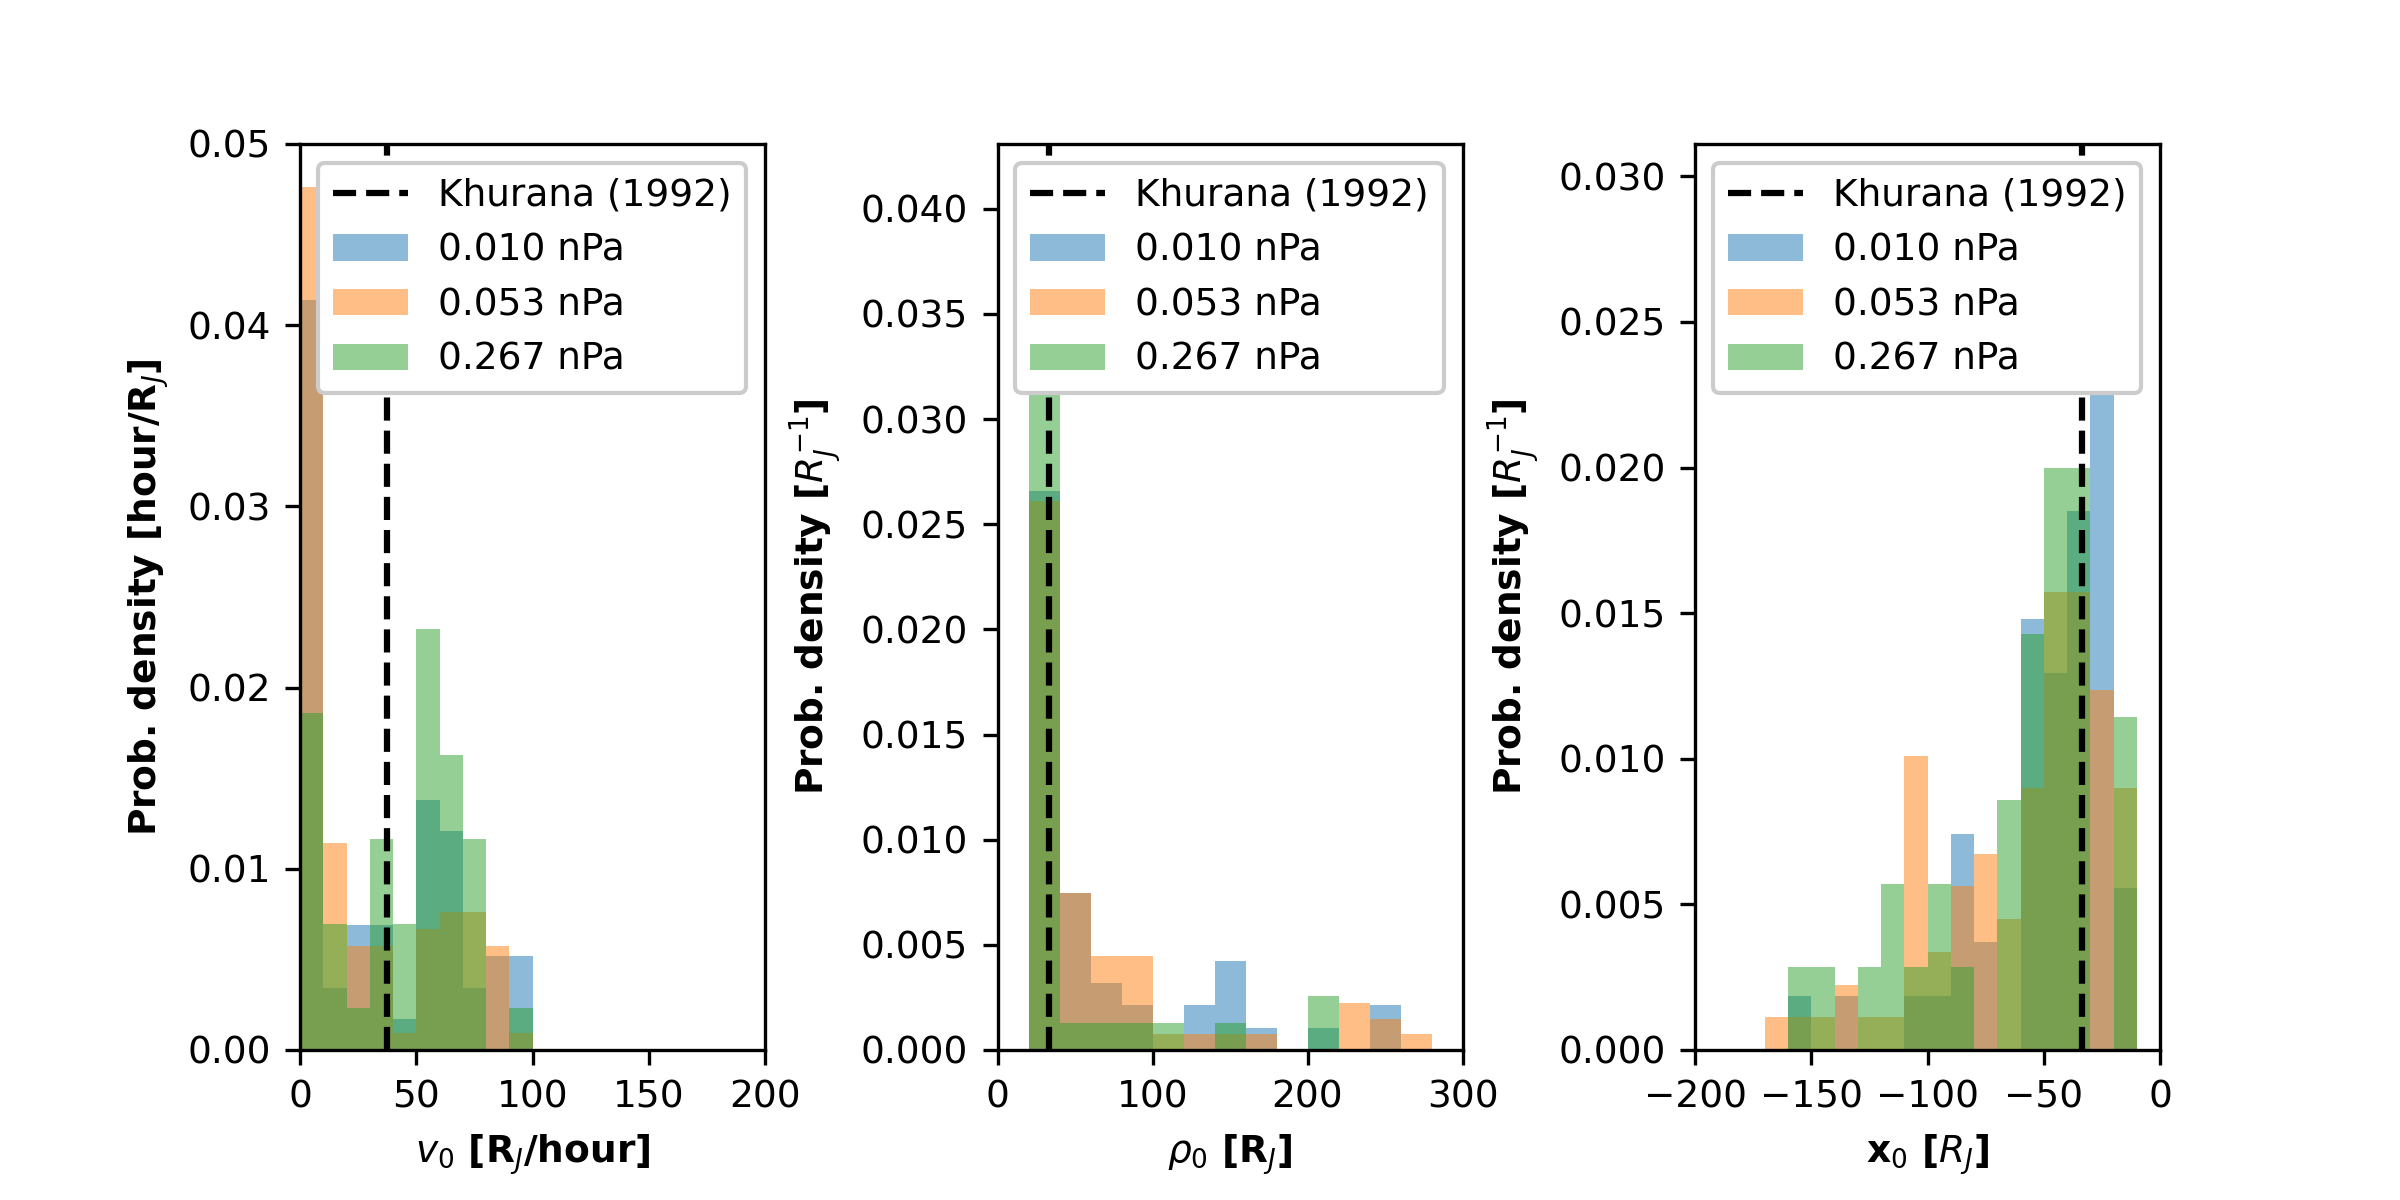
\includegraphics[width=\textwidth]{images5/comparison_highdynP_khurana.png}
    \caption{Histograms of the parameters used to fit the Khurana (1992) model form to the current sheet in the MHD model. Different colors represent the different solar wind dynamic pressures.}
    \label{fig:comparison-hist-khurana}
\end{figure}

\begin{table}
    \centering
    \begin{tabular}{c|c|c|c|c|c|c|c}
     $p_\text{dyn}$ &      $N$&  mean$(v_0)$&  median$(v_0)$&  mean$(\rho_0)$&    median($\rho_0$)& mean$(x_0)$&  median$(x_0)$\\
     nPa&   &   $R_J/$hour& $R_J/$hour& $R_J$   & $R_J$  &$R_J$  & $R_J$\\
     \hline
     0.01 &  58 &    34.08 &      28.90 &     137.03 &        52.62 &   -43.97 &     -36.49 \\
     0.05 & 105 &    26.16 &      12.09 &     210.03 &        87.48 &  -199.34 &     -49.41 \\
     0.27 &  43 &    43.25 &      50.84 &      78.23 &        22.10 &  -101.96 &     -46.13 \\
    \end{tabular}
    \caption{Statistics of the fits to the Khurana (1992) model shown in the histograms in Figure \protect\ref{fig:comparison-hist-khurana}. $N$ is the total number of good fits in each case.}
    \label{tab:comparison-khurana}
\end{table}

The model described by Equation \ref{eqn:khurana1992} contains three parameters - the asymptotic wave propagation speed $v_0$, the radial location where the current sheet wave starts to propagate $\rho_0$, and the characteristic hinging distance in the $x$-direction, $x_0$. Histograms of these parameters, which best fit the results from different times in the MHD simulation are shown in Figure \ref{fig:comparison-hist-khurana}. Since this model has three parameters, the least-squares minimization is less robust and leads to less `good' fits than the other models, which have only two parameters.

Unlike the previous three models, the asymptotic wave propagation speed $v_0$ does not show a preference and ranges between 0 to 100 $R_J$/hour. Unlike the previous models, which show a clear correlation between increasing solar wind dynamic pressure and decreasing wave speed, no correlation was seen in this model. The average speed for different solar wind dynamic pressures were found to be 34.08 $R_J$/hour (676.79 km/s), 26.16 $R_J$/hour (519.50 km/s) and 43.25 $R_J$/hour (858.89 km/s), which is close to the value obtained by \citeA{Khurana1992a} of 37.4 $R_J$/hour (742.7 km/s). 

As seen in the \citeA{Kivelson1978ASheet} model case, this model too favours low values of $\rho_0$, which can be seen in the histogram for all three dynamic pressure cases showing a strong peak at $\sim30$ $R_J$ However, there are more outliers in this case as shown in the higher values of the average compared to the median, which are 52.62 $R_J$, 87.48 $R_J$ and 22.10 $R_J$ for the three dynamic pressure cases respectively. In comparison, \citeA{Khurana1992a} obtain a value of $33.2$ $R_J$, which matches well with the peak of the distribution. 

The hinging distance $x_0$ shows a similar range as for the \citeA{Behannon1981} model, with the key difference being that $x_0$ is shown as negative values (as $x$ is negative in the magnetotail), whereas $a_0$ was applied to all longitudes and was a radial coordinate. The histogram of $x_0$ shows a preference for distances closer to the planet, but is spread over between -10 to -170 $R_J$ in the magnetotail. The mean of the distribution of the three solar wind dynamic pressure cases are $-43.97$ $R_J$, $-199.34$ $R_J$ and $-101.96$ $R_J$ respectively, whereas the median ranges from $-36.49$ $R_J$, $-49.41$ $R_J$ and $46.13$ $R_J$. These values match well the result by \citeA{Khurana1992a}, who found $x_0$ to be $-33.5$ $R_J$. There is considerable overlap between the histograms in all three cases, and no clear correlation can be identified between the value of $x_0$ and solar wind dynamic pressure. 

Overall, the \citeA{Khurana1992a} gives values which are reasonable, but the different behaviour of $v_0$ compared to the previous models hints that the minimization process was less robust when the number of parameters to fit was increased. In all cases discussed above, the considerable spread in the hinging parameter ($a_0$ for the \citeNP{Behannon1981} case and $x_0$ for the \citeNP{Khurana1989OnStructure} case), and its insensitivity to the solar wind dynamic pressure, compared to the relatively less spread in the wave propagation speed ($U$ and $v_0$) suggests that the wave speed plays a more important role in determining the current sheet structure. 

\subsection{Changes in plasma parameters due to solar wind driven compression}

In Figures \ref{fig:chp5-comparison-slices-density}-\ref{fig:chp5-comparison-slices-magnetosonic}, we show contours of different plasma parameters such as mass density, temperature, magnetic field strength, and the Alfven, sound and magnetosonic speeds to understand how solar wind dynamic pressure influences wave speeds in the magnetosphere. All figures are split into two columns; the left column shows the YZ plane (dawn-dusk meridian) whereas the right column shows the XZ plane (noon-midnight) meridian. The current sheet (where $B_r=0$) is highlighted in each figure as a white line. Different rows represent the three different solar wind dynamic pressures in increasing order as shown in Table \ref{tab:sw-conditions-chp5}. All plots were made at a time when the magnetic moment of the dipole was entirely in the XZ plane and pointed sunward. 

\begin{figure}
    \centering
    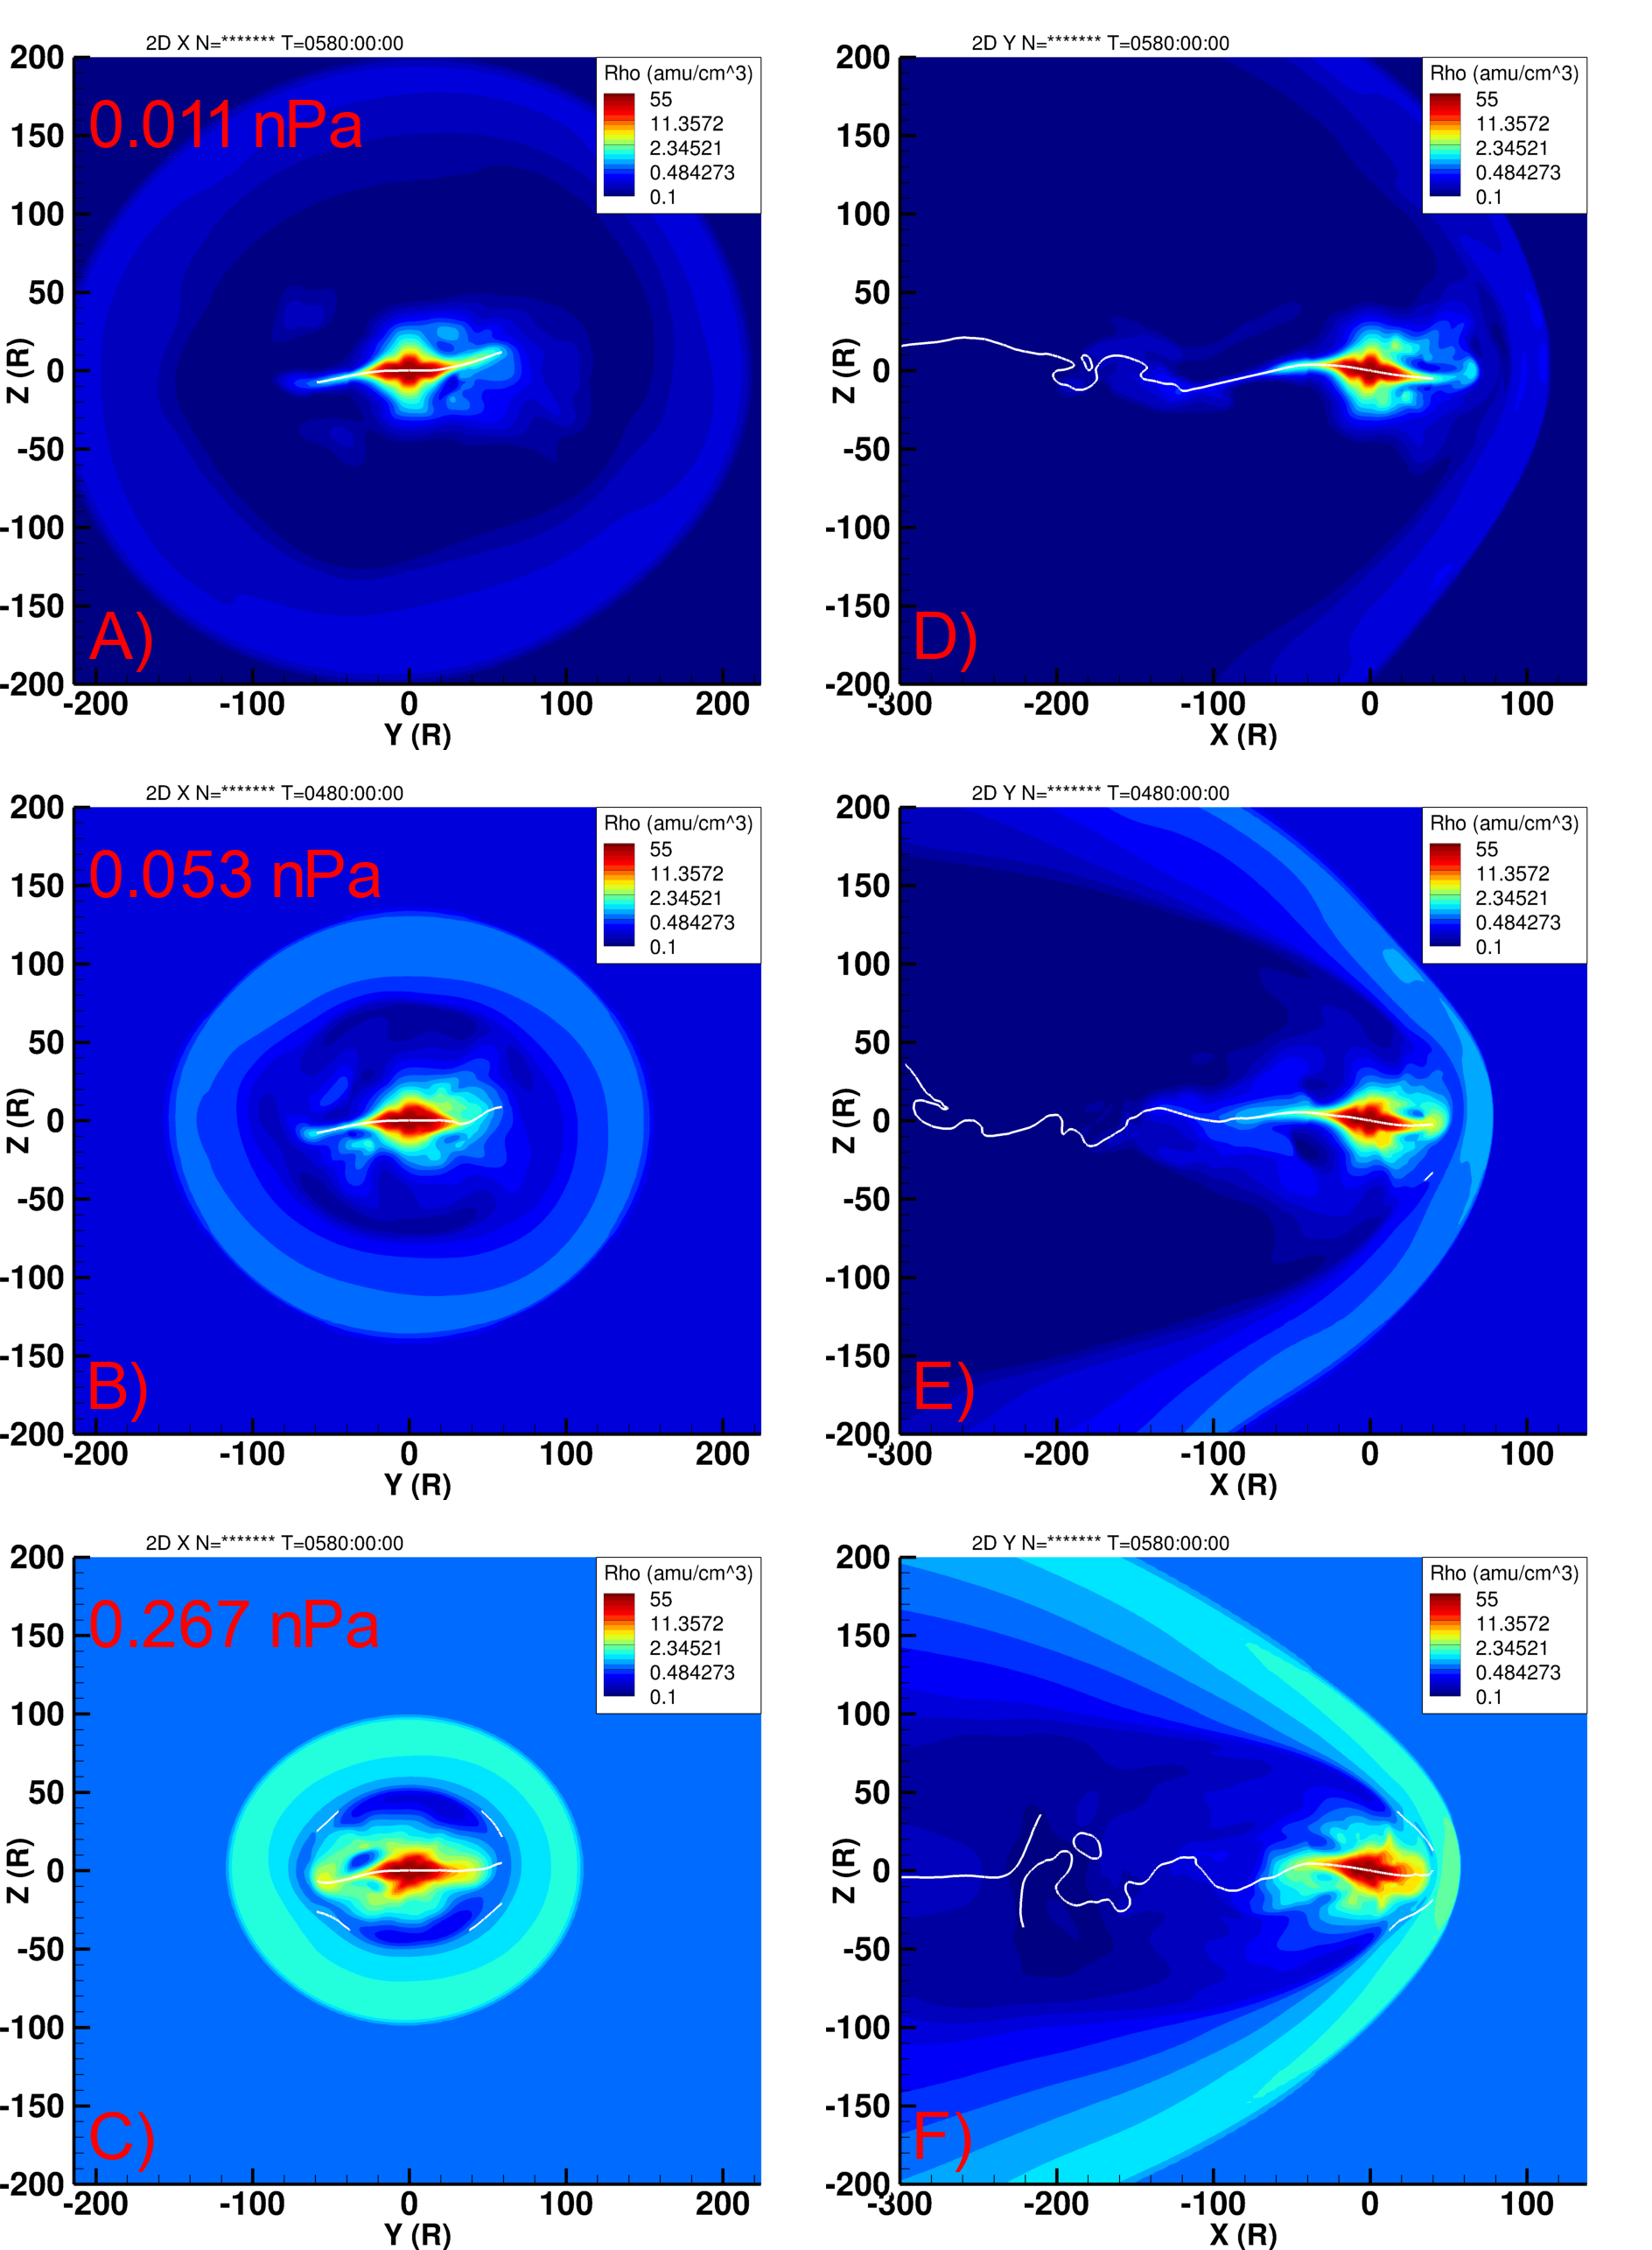
\includegraphics[height=0.9\textheight]{images5/compare_runs_currentsheet_Density.png}
    \caption{Plasma mass density contours in the $x=0$ (YZ) plane (A-C) and in the $y=0$ (XZ) plane (D-F) for different solar wind dynamic pressures. The current sheet is highlighted as a solid white curve.}
    \label{fig:chp5-comparison-slices-density}
\end{figure}

Figure \ref{fig:chp5-comparison-slices-density} shows the contours of plasma density $\rho_m$ in units of amu/cm$^3$. As expected, the magnetosphere is compressed and reduces in size as the solar wind dynamic pressure is increased, which can be seen by identifying the bow shock and magnetopause regions as two discontinuities characterized by sharp density gradients. The density in the magnetosphere also increases drastically in the magnetosheath, but also increases in the other regions of the magnetosphere, including its deep interior (panel F). Note particularly the magnetotail lobe regions surrounding the current sheet (white curve), which have a density of $\sim0.1$ amu/cm$^3$ for the 0.011 nPa case and which increases to $>2$ amu/cm$^3$ for the 0.267 nPa solar wind dynamic pressure case. 

One can also see the different behaviour of the current sheet in panels D, E and F of Figure \ref{fig:chp5-comparison-slices-density} (solid white curve). For the 0.011 nPa case, the current sheet oscillations appear more gradual, and a minima and maxima are separated by $\sim200$ $R_J$. In constrast, for the 0.267 nPa case, the current sheet oscillates more strongly, with a maxima and minima separation (or the effective half-wavelength) of only about $50$ $R_J$. In panel F, at around $x=-200$ $R_J$ the oscillations of the current sheet break into disjoint curves, which are a result of plasmoid generation due to magnetic reconnection.  

\begin{figure}
    \centering
    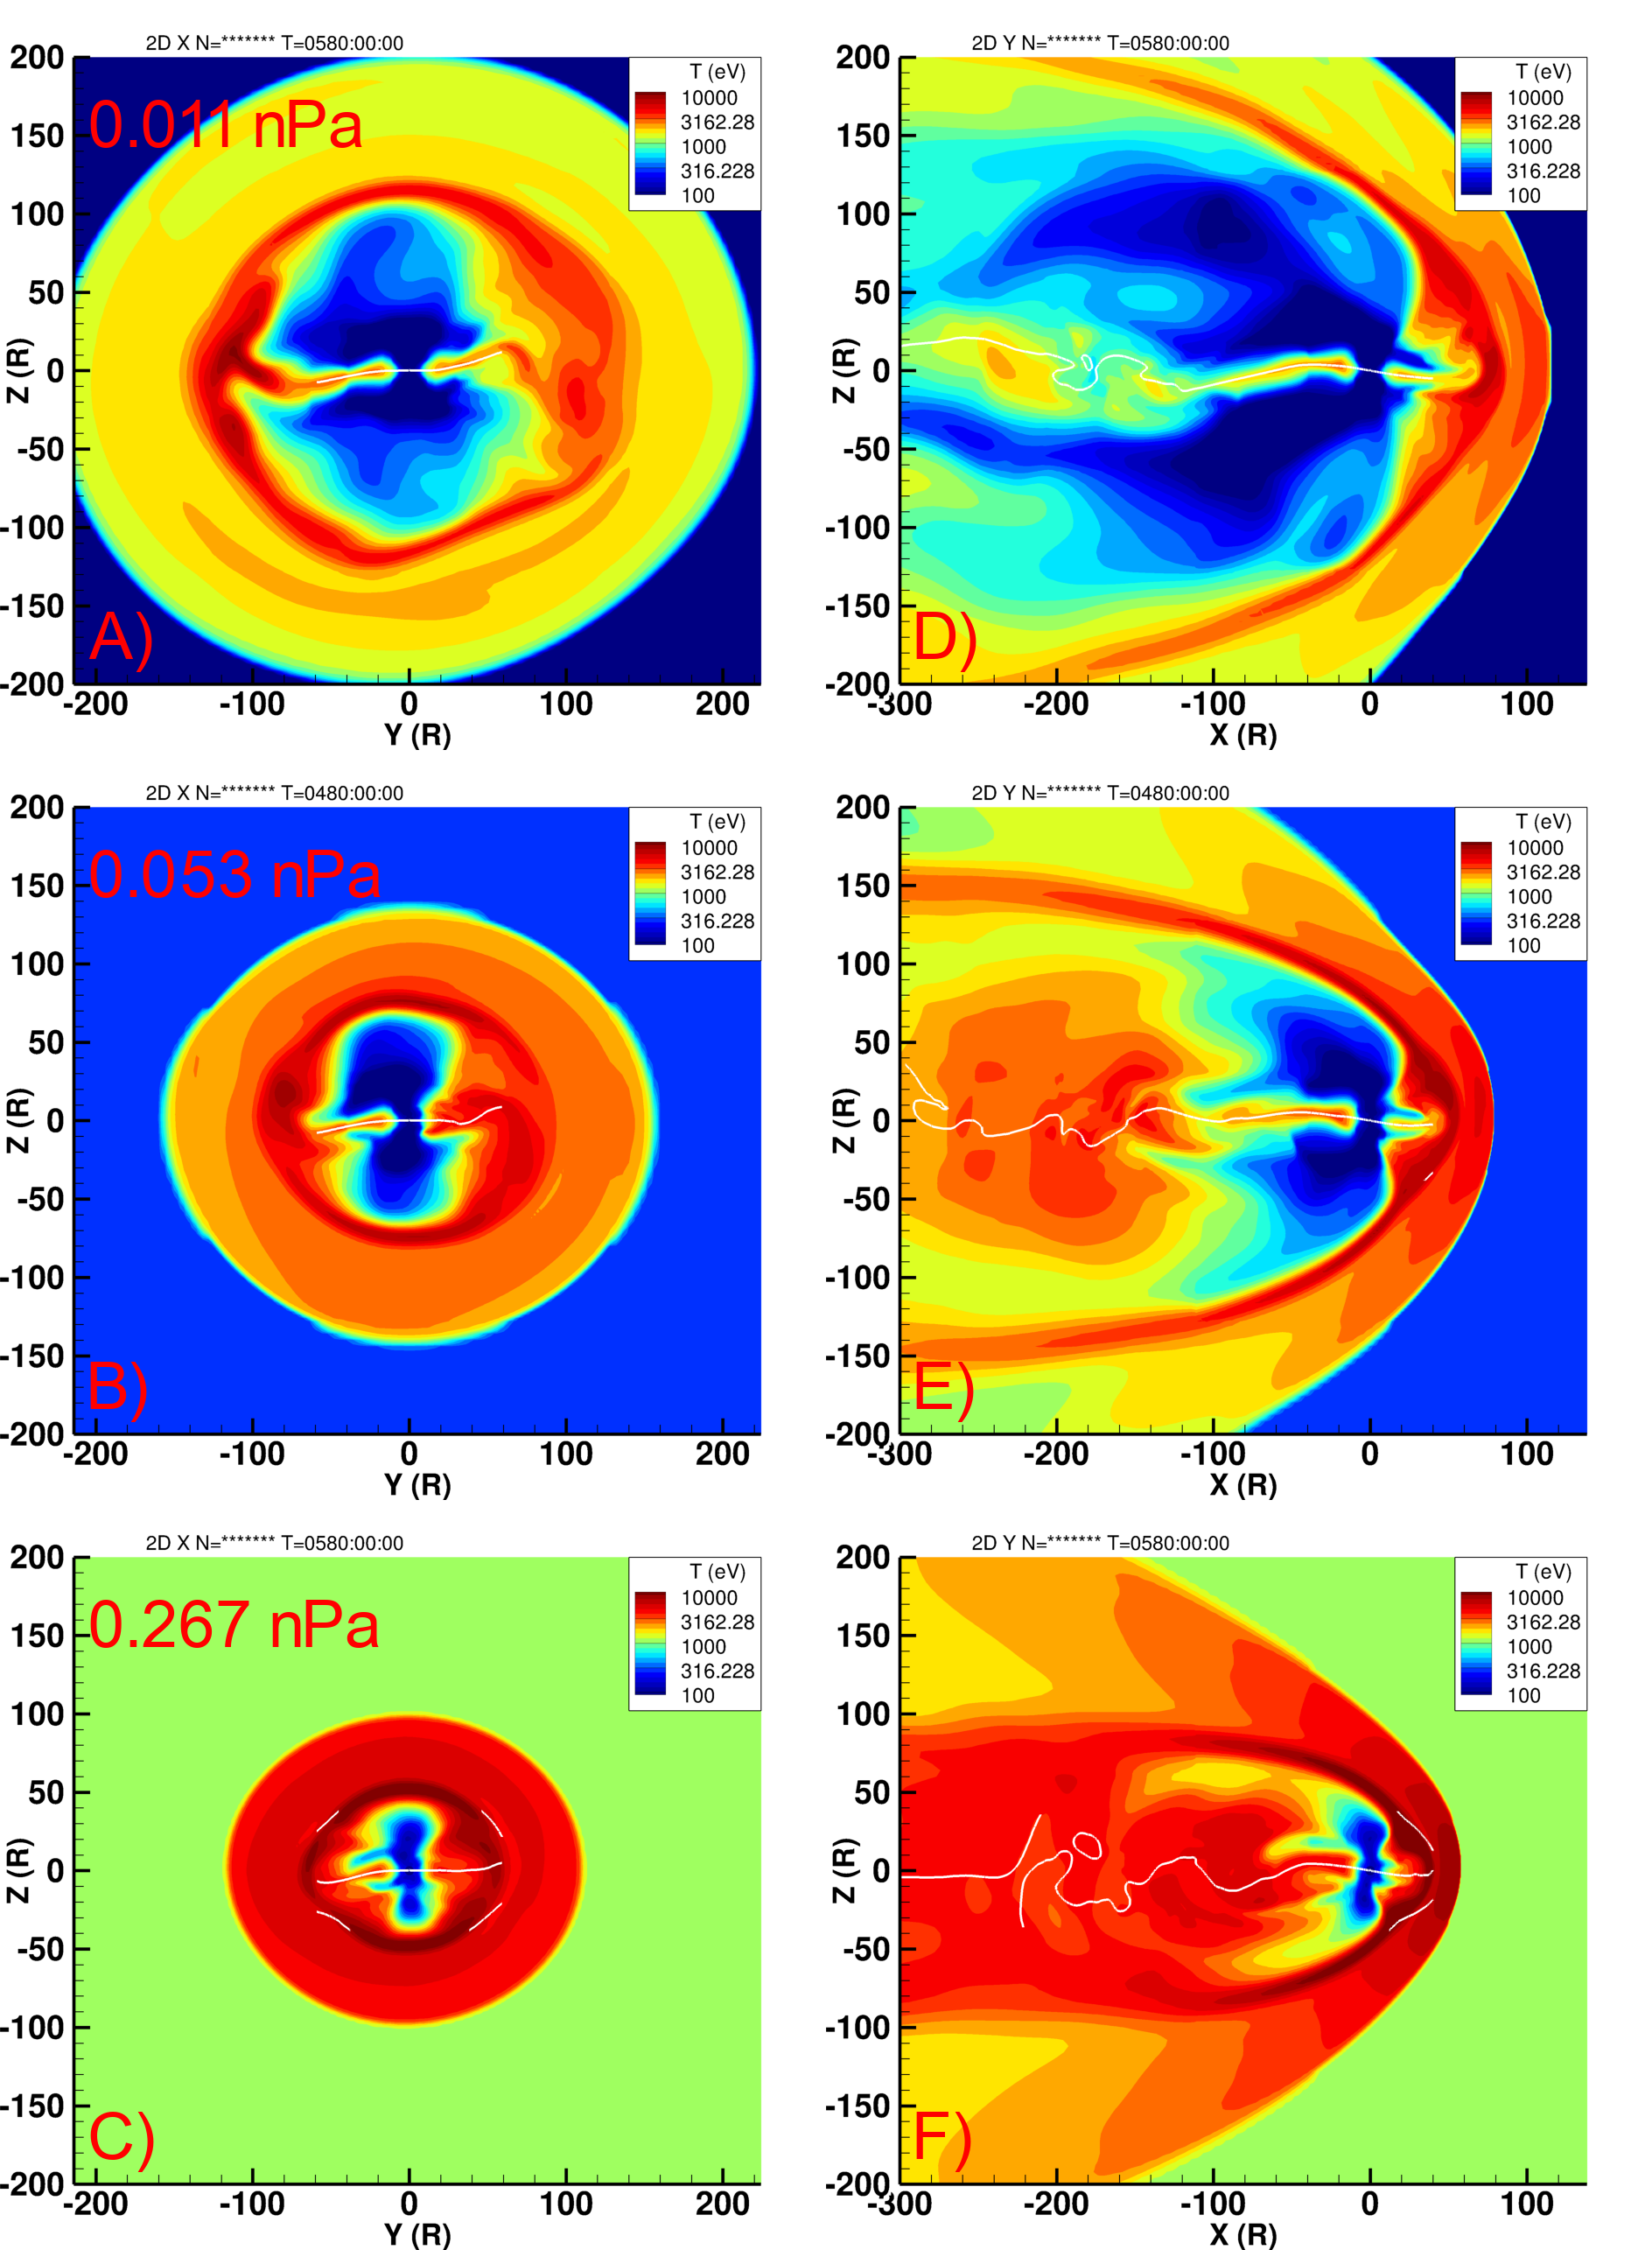
\includegraphics[height=0.9\textheight]{images5/compare_runs_currentsheet_Temperature.png}
    \caption{Contours of plasma temperature in the $x=0$ (YZ) plane (A-C) and in the $y=0$ (XZ) plane (D-F) for different solar wind dynamic pressures. The current sheet is highlighted as a solid white curve.}
    \label{fig:chp5-comparison-slices-temperature}
\end{figure}

In Figure \ref{fig:chp5-comparison-slices-temperature}, we show the contours of plasma temperature $T = p/nk_B$ in eV, assuming an ion mass of 16 amu. As expected, a larger solar wind dynamic pressure creates a stronger bow shock and increases the temperature in the magnetosheath regions. However, we also find that despite an increase in density (as seen in Figure \ref{fig:chp5-comparison-slices-density}), the plasma temperature in the magnetotail increases by almost two orders of magnitude between the case of 0.011 nPa and 0.267 nPa, from 100 eV to $\sim$5000 eV, for e.g. at $x=-200$ $R_J$. This increase in plasma temperature is also seen in the magnetotail lobes (panels D, E and F), which we discussed previously as having increased in density by a factor of 10 to 20 due to the solar wind compression. 


\begin{figure}
    \centering
    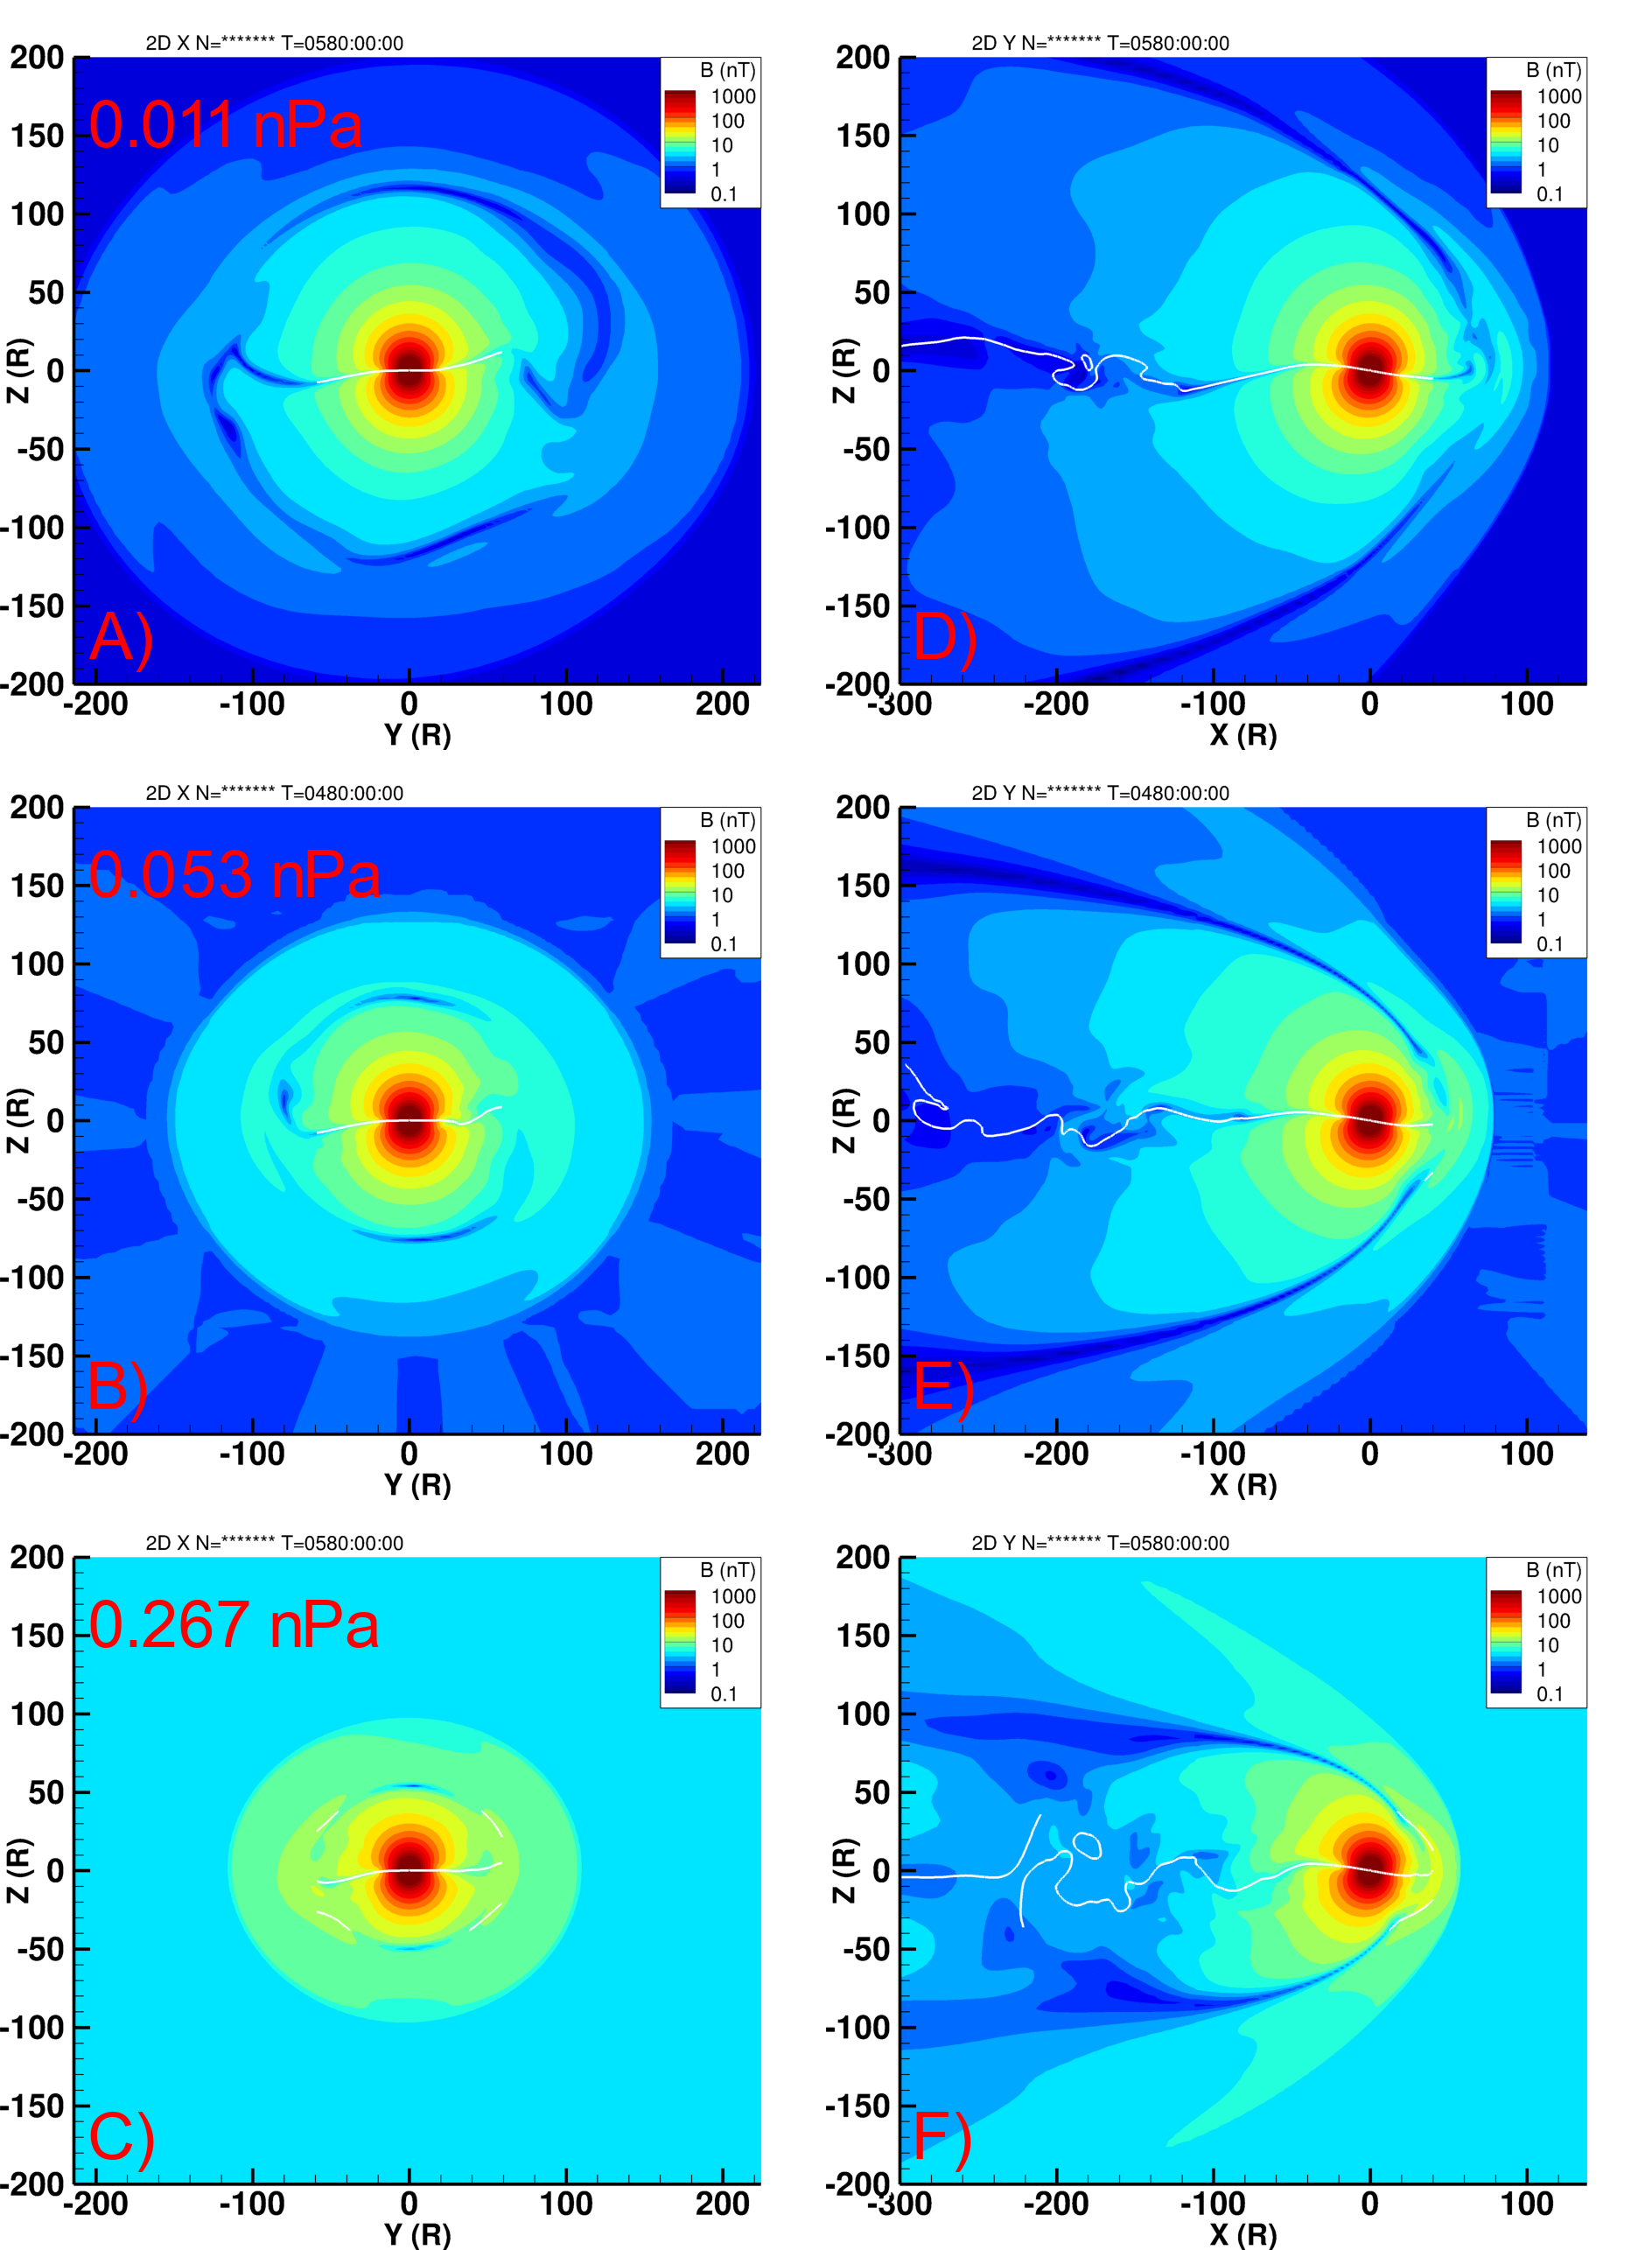
\includegraphics[height=0.9\textheight]{images5/compare_runs_currentsheet_Bmag.png}
    \caption{Magnetic field strength contours in the $x=0$ (YZ) plane (A-C) and in the $y=0$ (XZ) plane (D-F) for different solar wind dynamic pressures. The current sheet is highlighted as a solid white curve.}
    \label{fig:chp5-comparison-slices-Bmag}
\end{figure}

In Figure \ref{fig:chp5-comparison-slices-Bmag}, we show contours of the magnetic field strength in nT. Unlike the previous cases for density and temperature, the magnetic field does not exhibit drastic changes due to the solar wind compression. However, an increase in field strength can be seen in panels D, E and F in the magnetotail lobes, e.g. at $x=-100$ $R_J$ and $z=-50$ $R_J$, likely due to the increased magnetic pressure in the lobes to balance the higher solar wind dynamic pressure outside the magnetopause. 

\begin{figure}
    \centering
    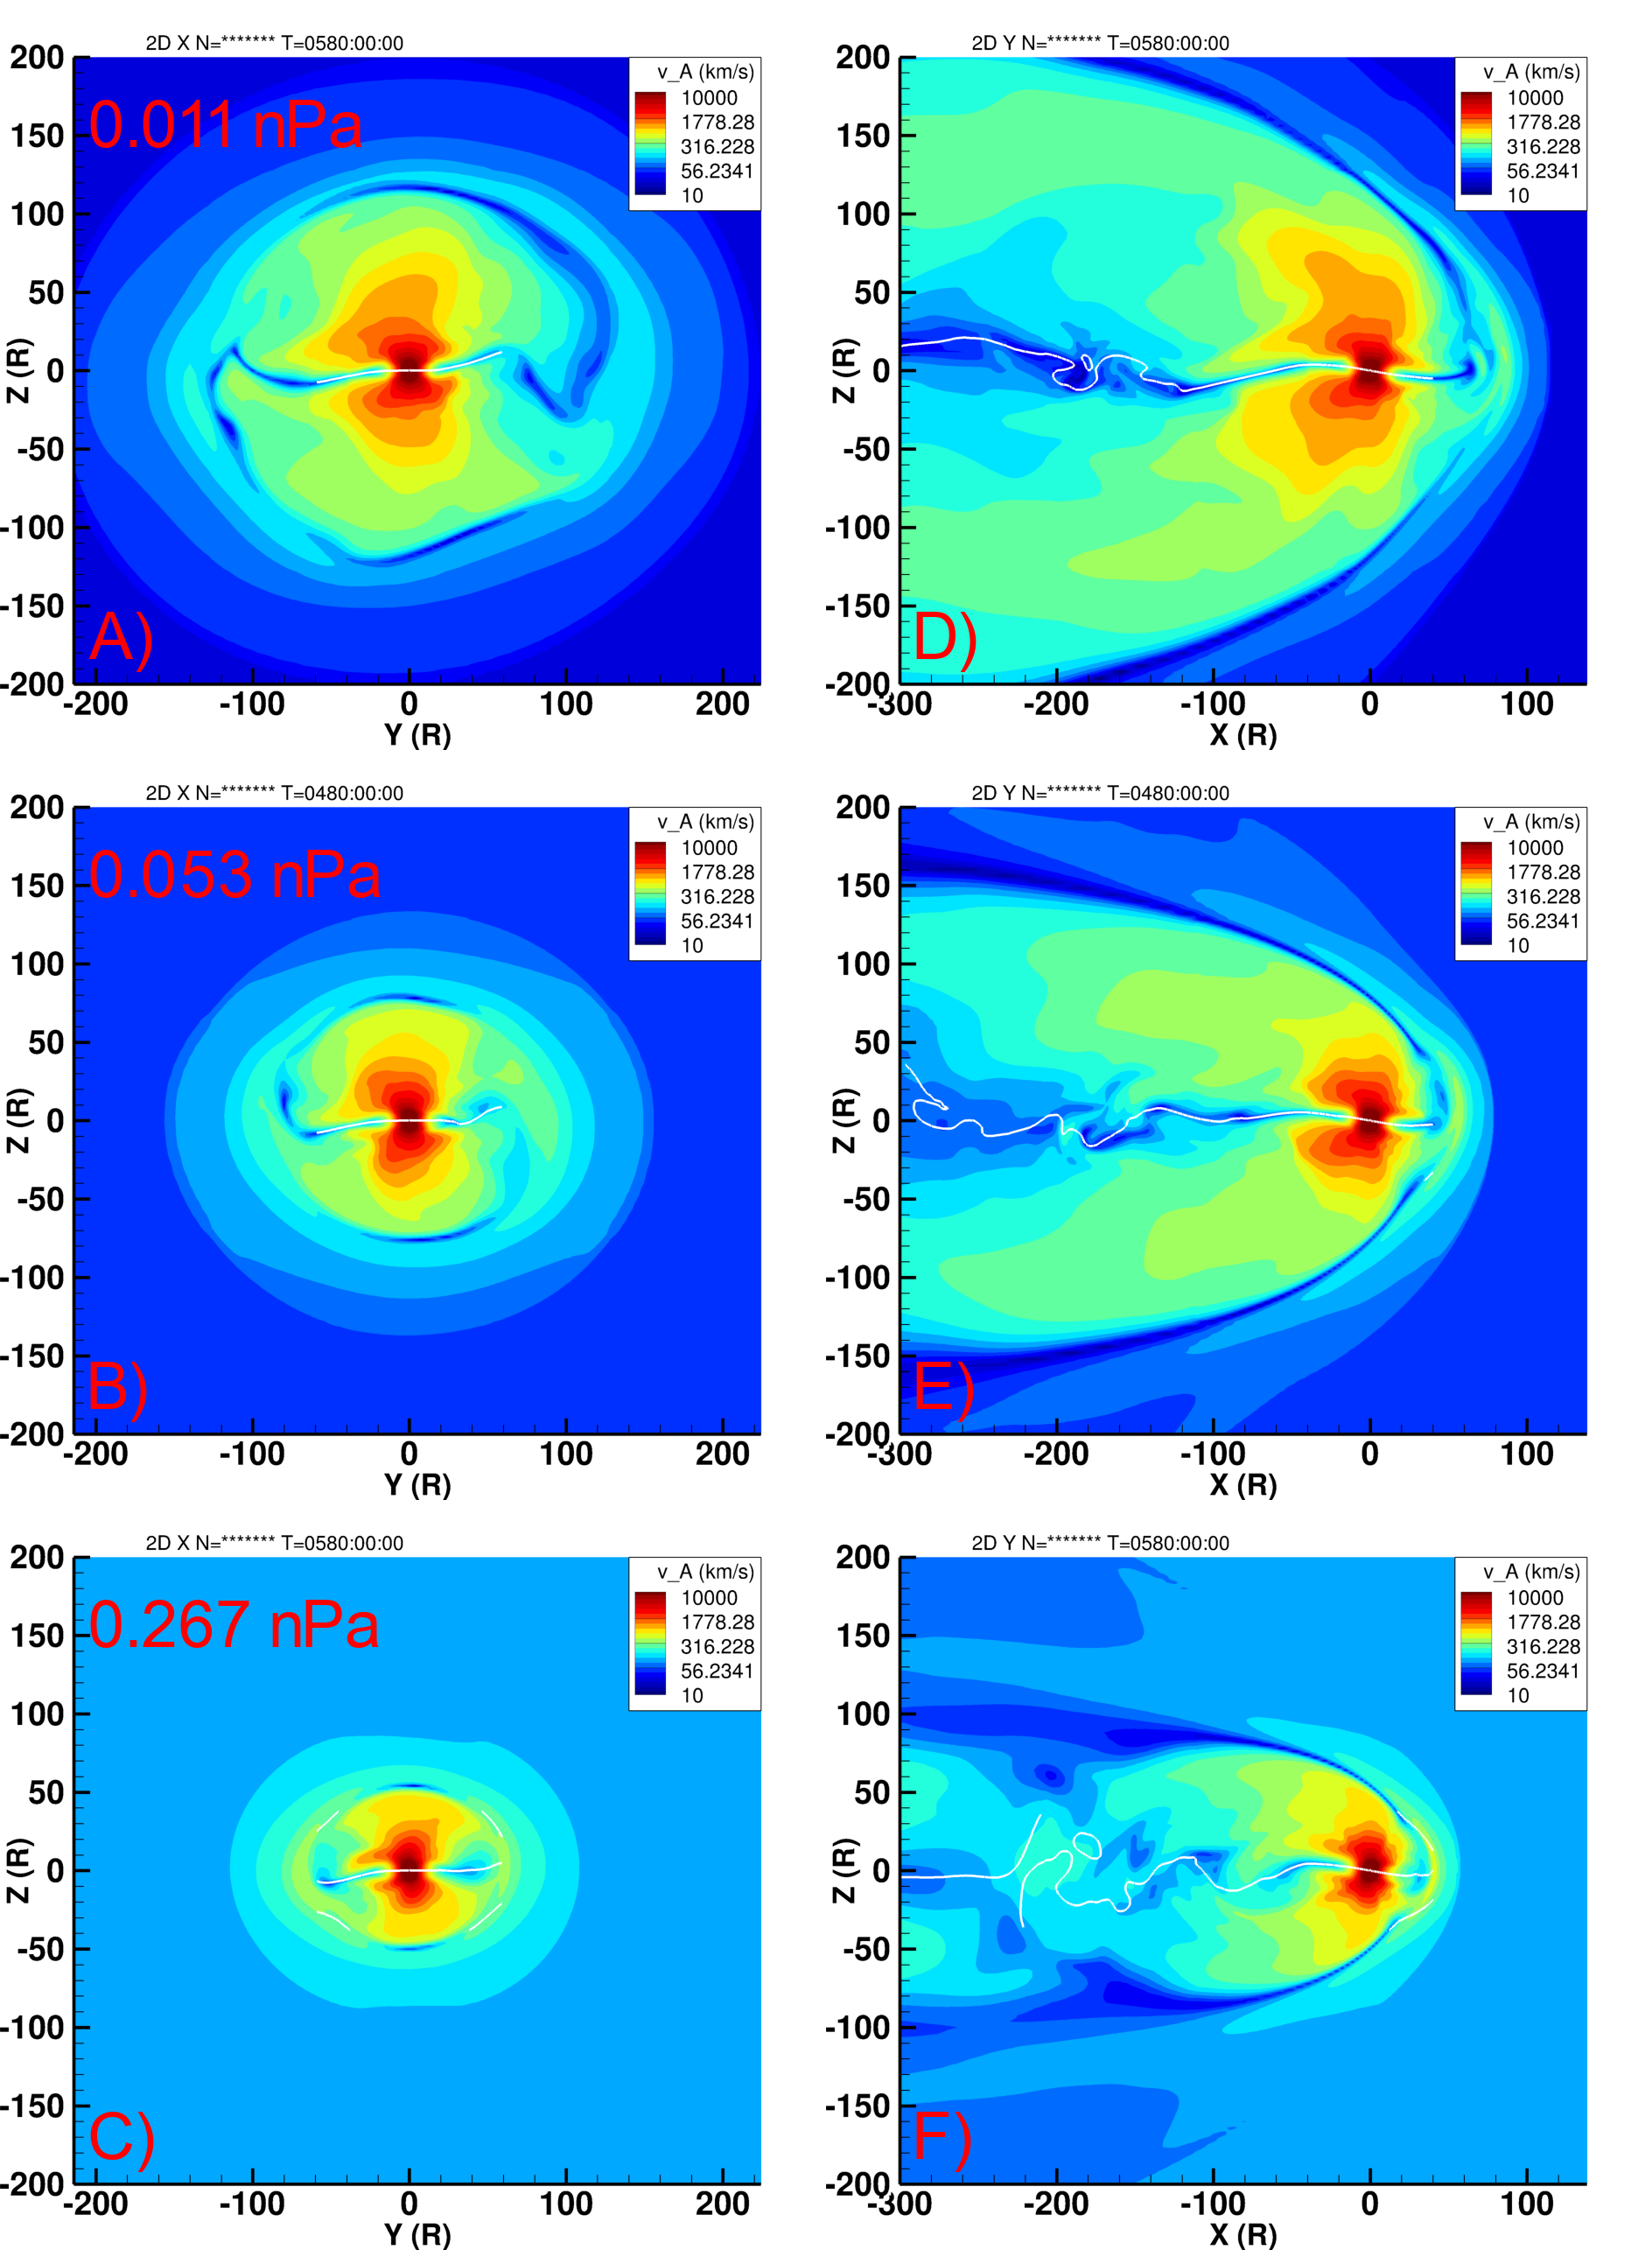
\includegraphics[height=0.9\textheight]{images5/compare_runs_currentsheet_AlfvenSpeed.png}
    \caption{Alfven speed contours in the $x=0$ (YZ) plane (A-C) and in the $y=0$ (XZ) plane (D-F) for different solar wind dynamic pressures. The current sheet is highlighted as a solid white curve.}
    \label{fig:chp5-comparison-slices-alfven}
\end{figure}

Knowing the magnetic field strength and plasma density, we can estimate the Alfven speeds in the MHD simulation. Its contours are shown in Figure \ref{fig:chp5-comparison-slices-alfven} in units of km/s. Since the Alfven speed is propotional to $B$ but inversely proportional to $\rho^{1/2}$, we expect the contours to follow that of the magnetic field closely. The smallest Alfven speed in the magnetotail are found at the current sheet, where the magnetic field is weak. The results from our MHD simulation clearly show that Alfven speeds in the magnetotail lobes, surrounding the current sheet, reduce due to a solar wind compression. For e.g. at the same location at $x=-100$ $R_J$ and $z=-50$ $R_J$, the Alfven speed reduces from $\sim316$ km/s to $\sim200$ km/s as the solar wind dynamic pressure is increased from 0.011 nPa to 0.267 nPa. The region of high Alfven speed, highlighted via red contours, is seen to shrink with increased solar wind dynamic pressure. This counter-intuitive result can be explained by the relative changes in $B$ and $\rho$; the increase in plasma density during the 0.267 nPa case is much larger than the corresponding increase in magnetic field strength in the magnetotail lobes. 

\begin{figure}
    \centering
    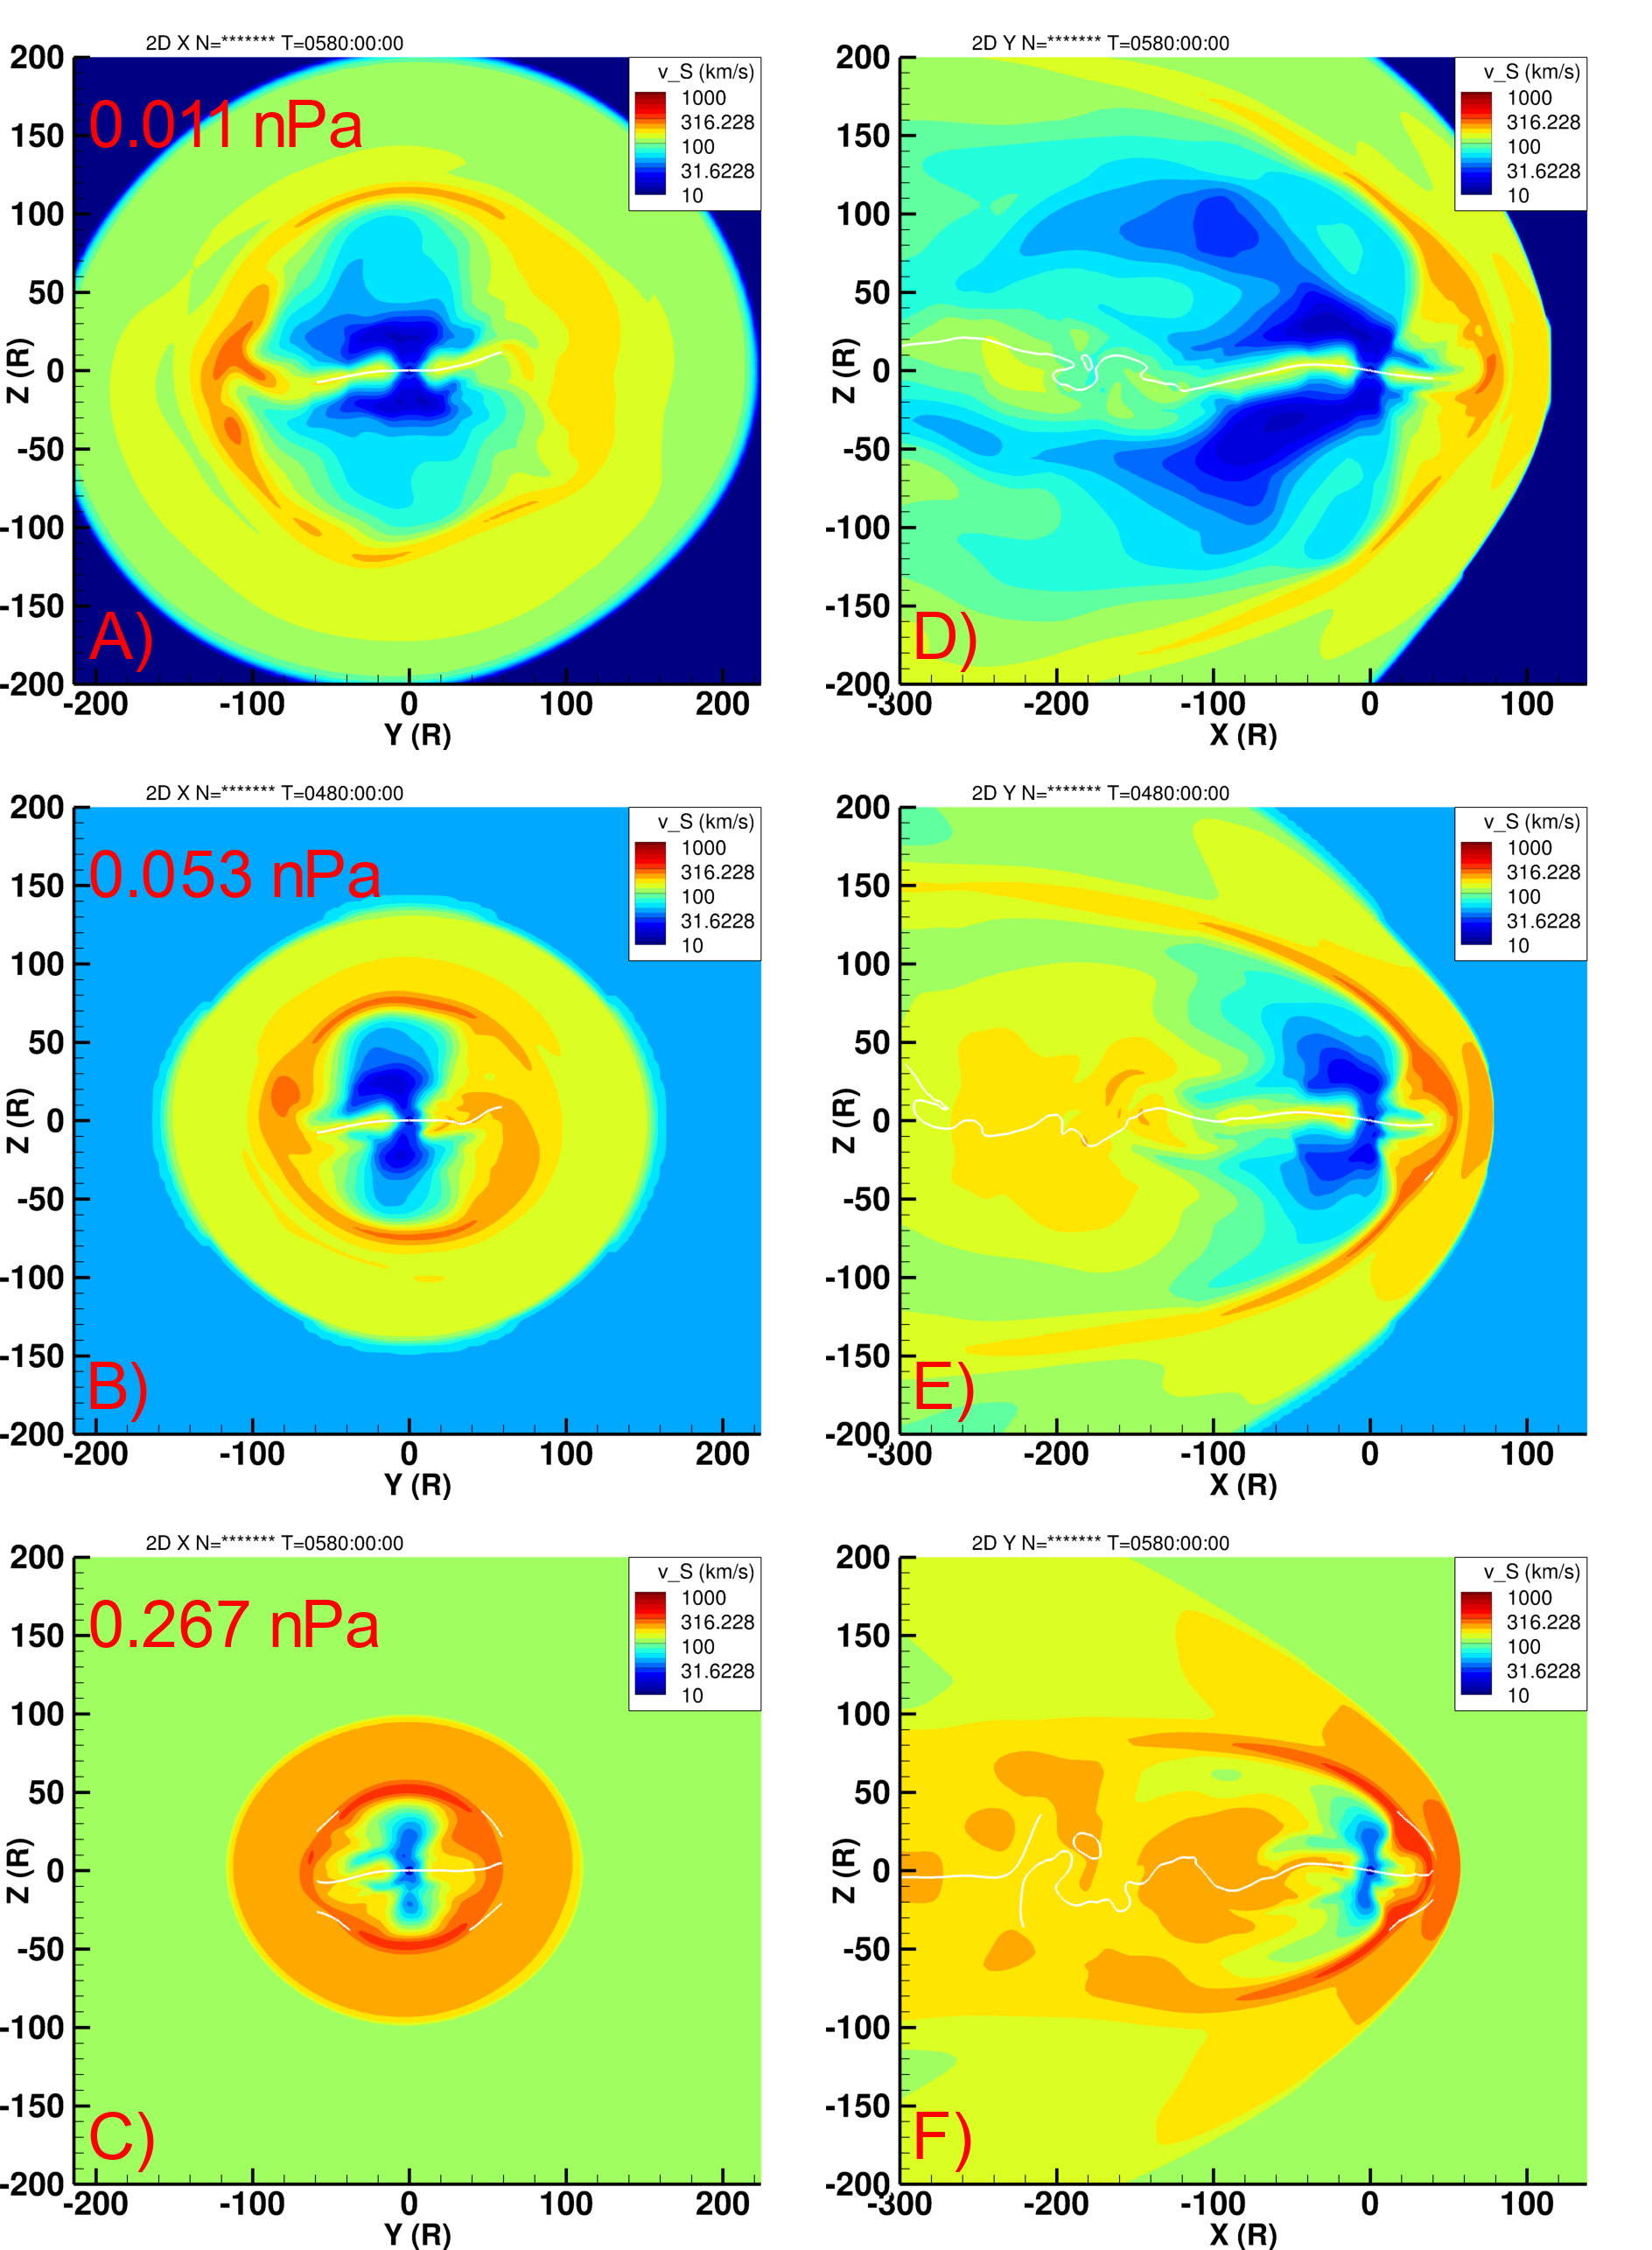
\includegraphics[height=0.9\textheight]{images5/compare_runs_currentsheet_SoundSpeed.png}
    \caption{Contours of the sound speed in the $x=0$ (YZ) plane (A-C) and in the $y=0$ (XZ) plane (D-F) for different solar wind dynamic pressures. The current sheet is highlighted as a solid white curve.}
    \label{fig:chp5-comparison-slices-sound}
\end{figure}

The sound speed can also be estimated from the model using the plasma pressure and density, and its contours are shown in Figure \ref{fig:chp5-comparison-slices-sound}. Unlike the Alfven speed, which is smallest at the current sheet, the sound speed inside the current sheet and associated plasma sheet is seen to be greater than in the surrounding magnetotail lobes. Increasing solar wind dynamic pressure increases the sound speed in all regions of the magnetosphere, which is expected as it is closely related to the plasma temperature, which we discussed increased by two orders of magnitude between the 0.011 nPa and 0.267 nPa case (Figure \ref{fig:chp5-comparison-slices-temperature}). 

\begin{figure}
    \centering
    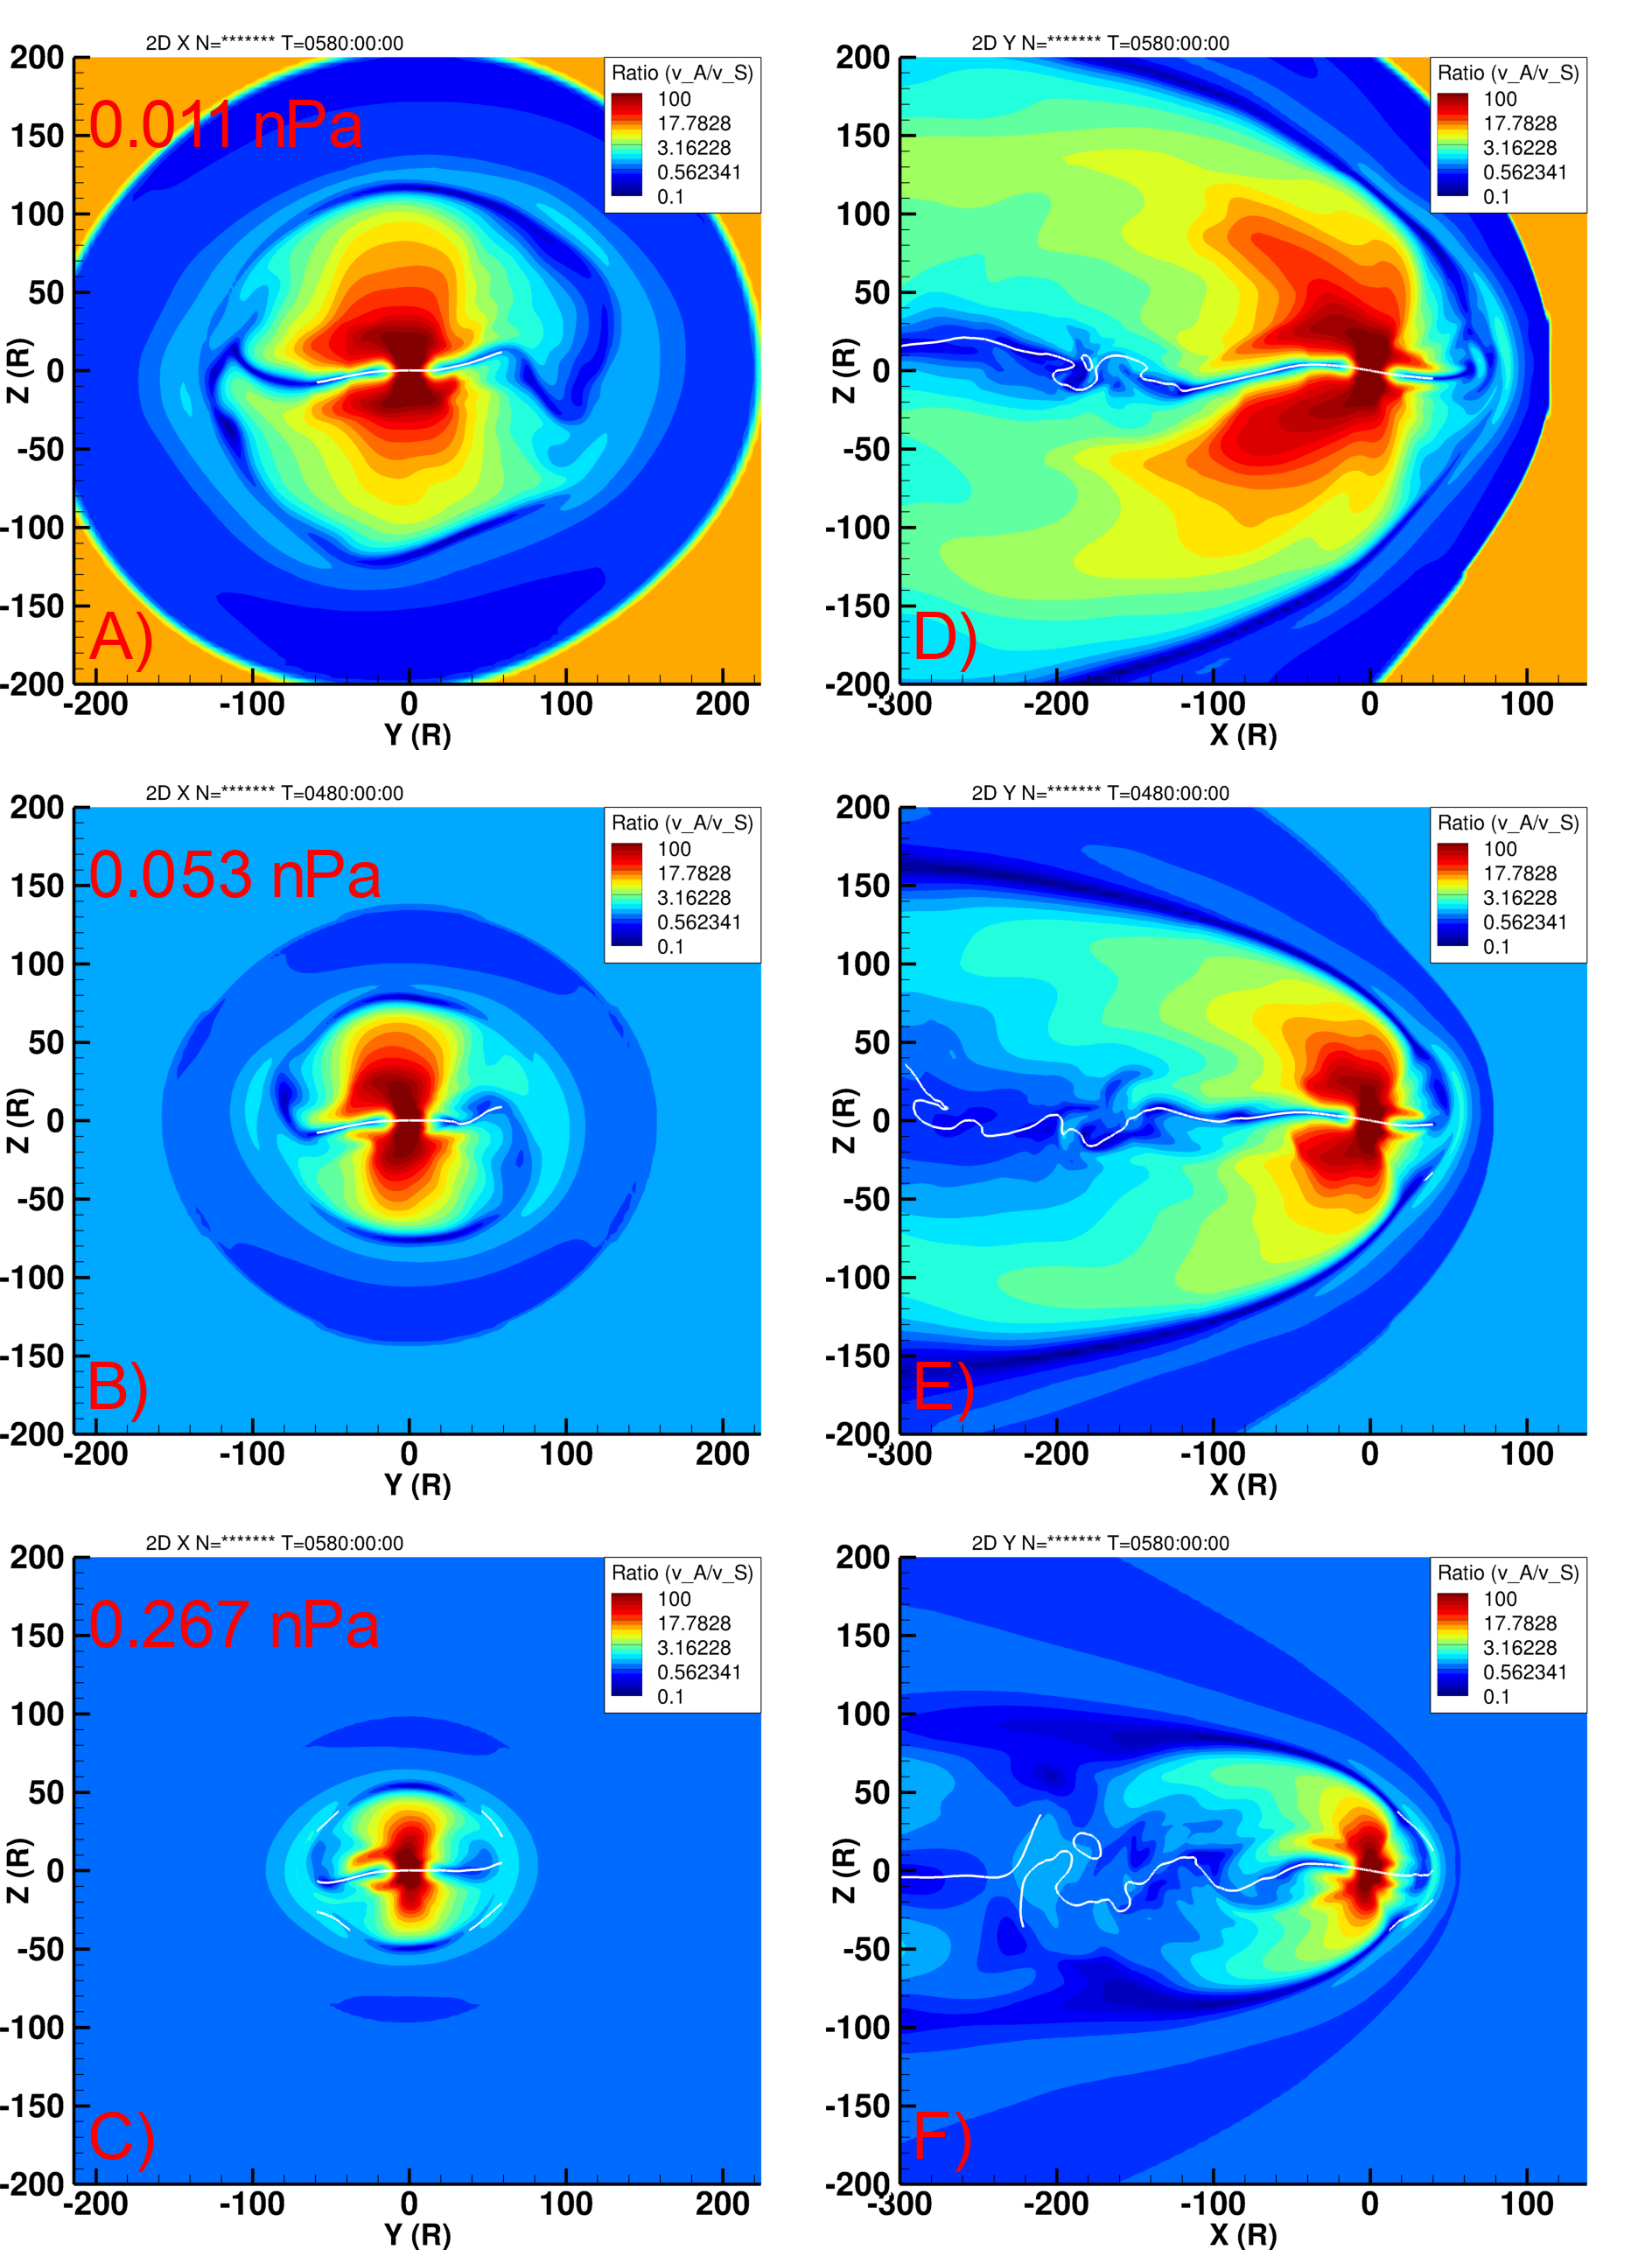
\includegraphics[height=0.9\textheight]{images5/compare_runs_currentsheet_RatioAlfvenSonic.png}
    \caption{Contours of the ratio of the Alfven speed to the sound speed in the $x=0$ (YZ) plane (A-C) and in the $y=0$ (XZ) plane (D-F) for different solar wind dynamic pressures. The current sheet is highlighted as a solid white curve.}
    \label{fig:chp5-comparison-slices-ratioalfvensound}
\end{figure}

The Alfven speed in the magnetotail is seen to decrease with increasing solar wind dynamic pressure (Figure \ref{fig:chp5-comparison-slices-alfven}), whereas the sound speed is seen to increase (Figure \ref{fig:chp5-comparison-slices-sound}), and this diverging behaviour needs to be further investigated. In Figure \ref{fig:chp5-comparison-slices-ratioalfvensound}, we show the contours of the ratio of the Alfven speed to the sound speed. In the majority of the inner and middle magnetosphere, the Alfven speeds are high and are larger than the sound speed by 1 to 2 orders of magnitude. However, this characteristic of the magnetosphere changes for higher solar wind dynamic pressures. Panels D, E and F of Figure \ref{fig:chp5-comparison-slices-ratioalfvensound} clearly show that with increasing solar wind dynamic pressure, the ratio of the Alfven speed to the sound speed decreases in all regions of the magnetosphere. Some regions in the outer magnetosphere which were previously dominated by the Alfven speed ($v_A/v_S \approx 20$) for the 0.011 nPa case now have sound speeds larger than the Alfven speed ($v_A/v_S < 1$) for the 0.267 nPa case, e.g. at $x=100$ $R_J$ and $z=-50$ $R_J$. 

\begin{figure}
    \centering
    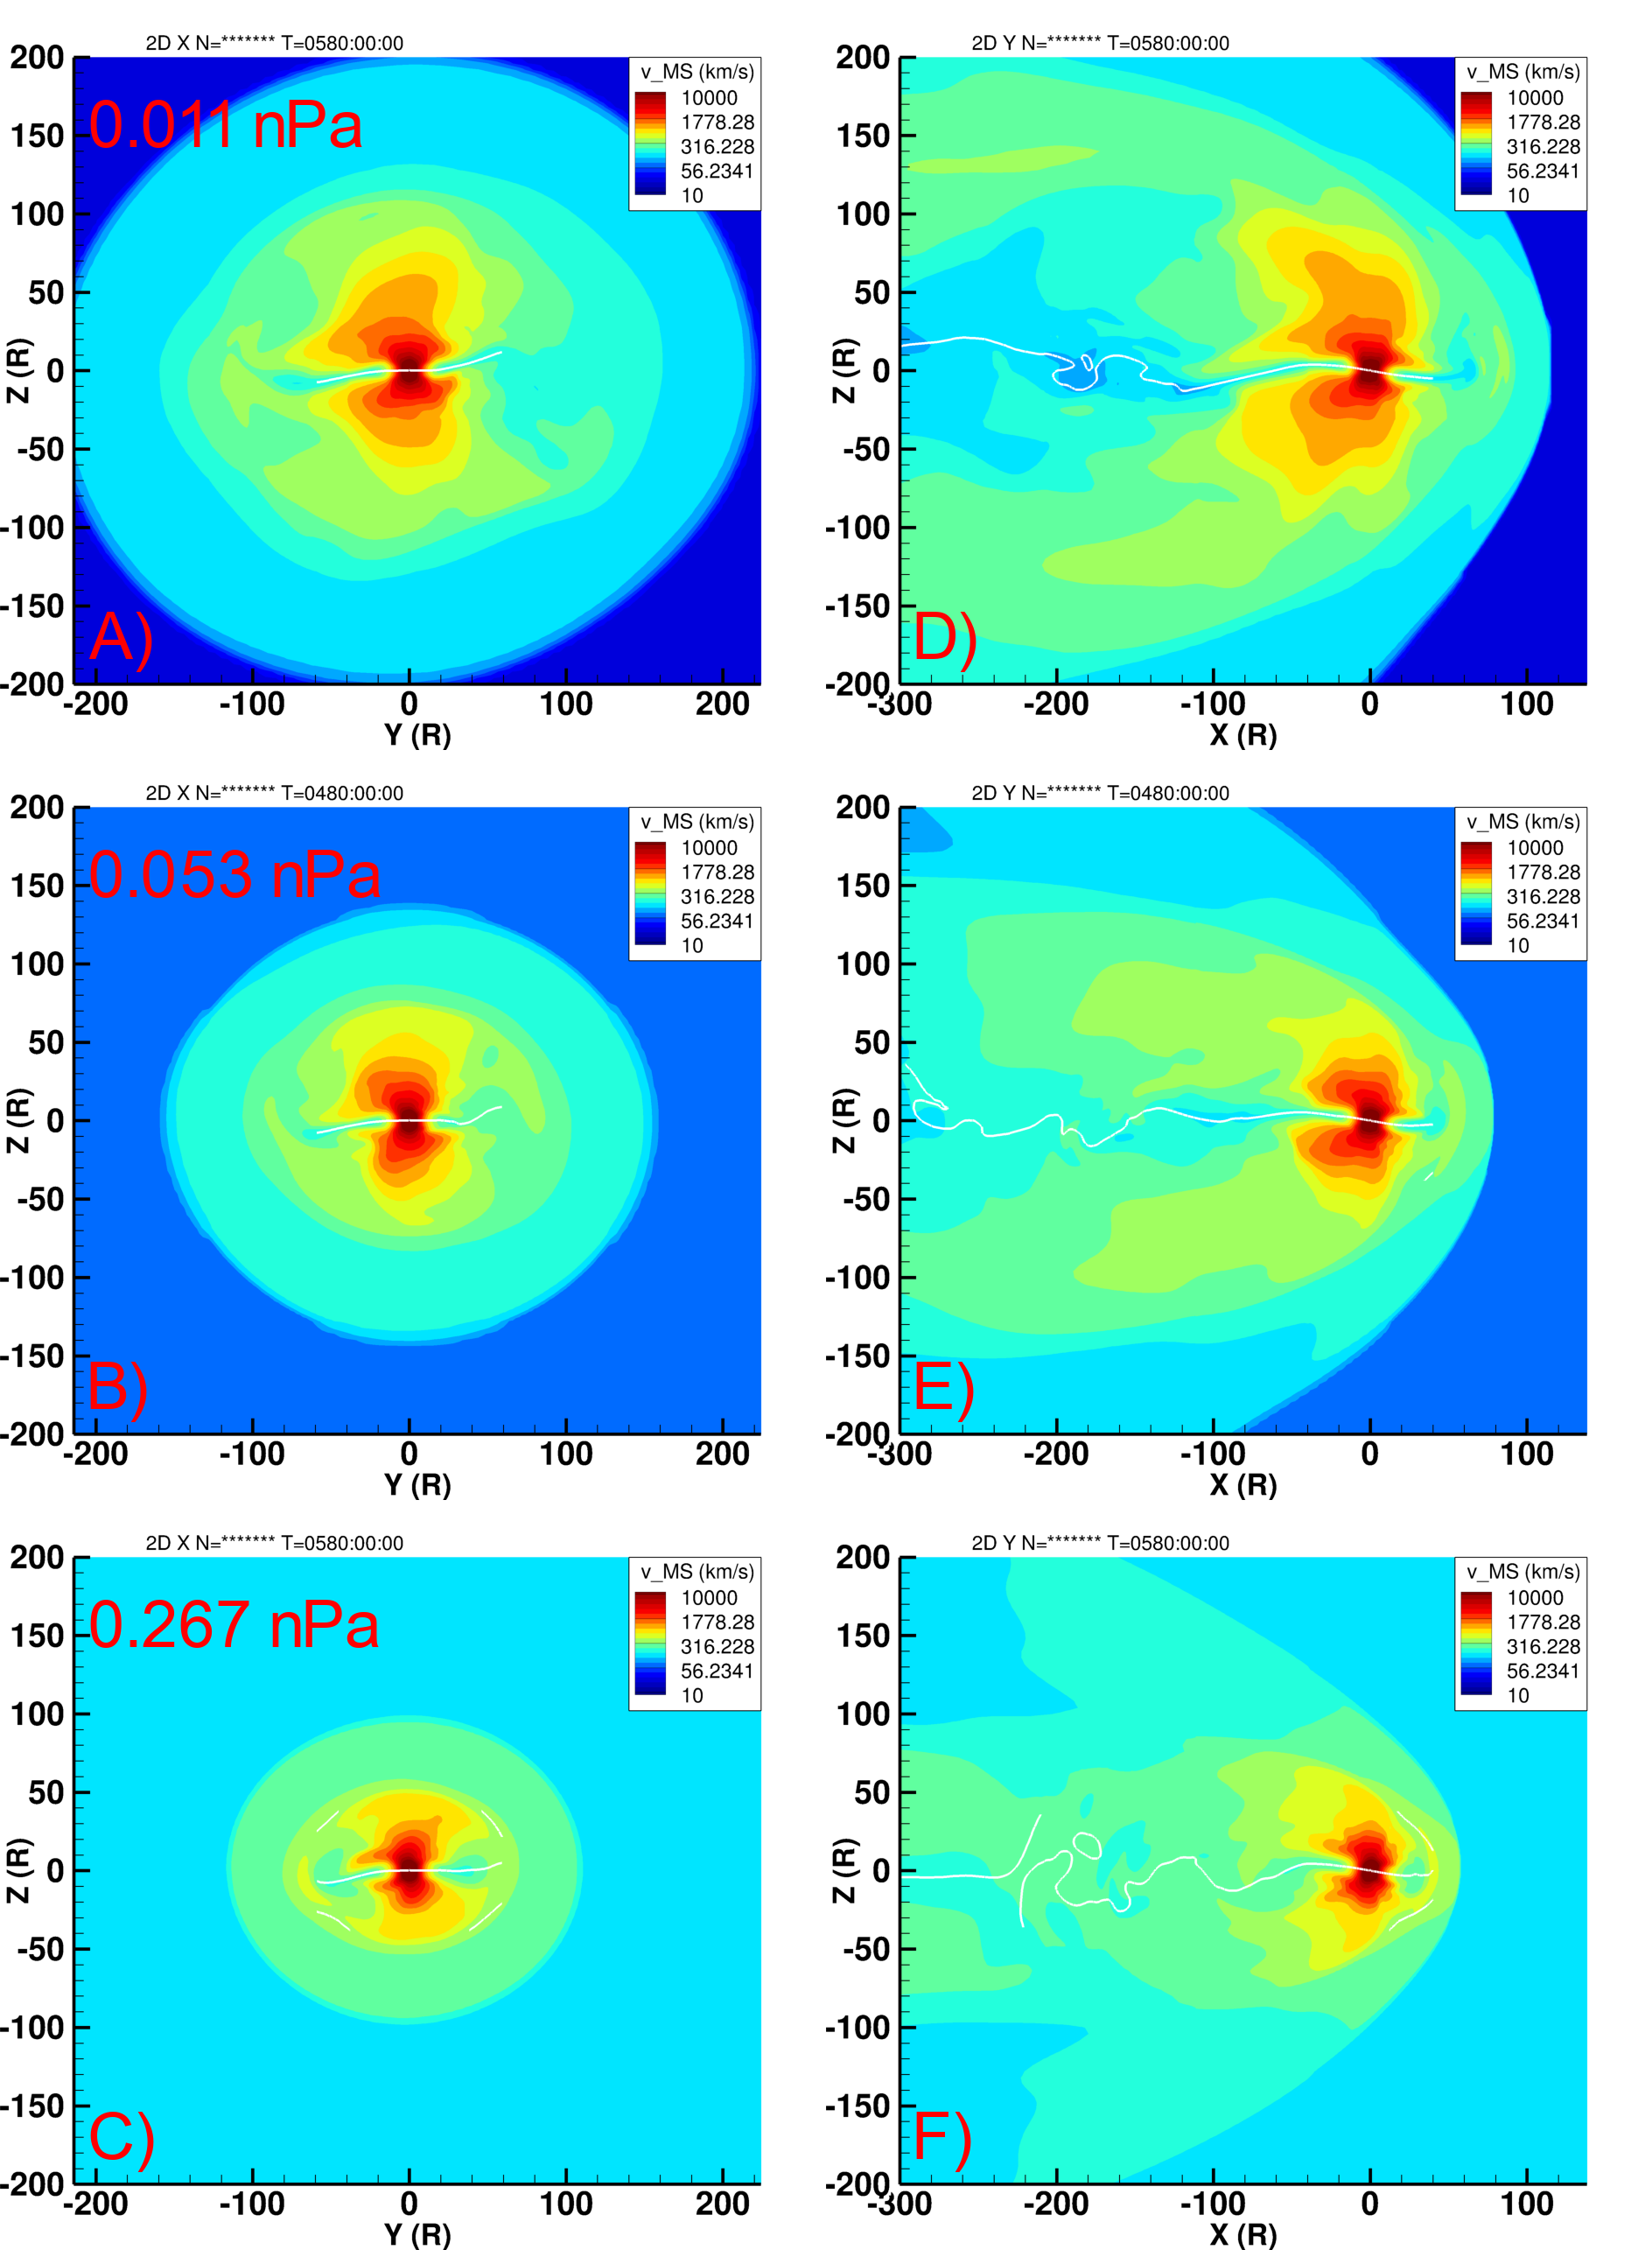
\includegraphics[height=0.9\textheight]{images5/compare_runs_currentsheet_MagnetosonicSpeed.png}
    \caption{Contours of the magnetosonic speed in the $x=0$ (YZ) plane (A-C) and in the $y=0$ (XZ) plane (D-F) for different solar wind dynamic pressures. The current sheet is highlighted as a solid white curve.}
    \label{fig:chp5-comparison-slices-magnetosonic}
\end{figure}

The fastest wave mode in the ideal MHD system is the fast magnetosonic mode, whose speed can be calculated using the Alfven and sound speeds ($v_\text{ms} = \sqrt{v_A^2 + v_S^2}$). The magnetosonic mode would represent the fastest means by which a location in the distant magnetotail would perceive a change in the orientation of the dipole, and hence is crucial to understand the oscillations of the current sheet. The contours of $v_\text{ms}$ are shown in Figure \ref{fig:chp5-comparison-slices-magnetosonic}, which can now be understood based on the changes in the individual components i.e. the Alfven speed and the sound speed, and ultimately the basic plasma properties such as density, temperature and magnetic field strength. 

Note that the wave speeds for semi-relativistic MHD do not have closed form expressions, so in these calculations we apply a simple correction to the conventional wave speeds as $v := \gamma v$ where $\gamma = 1/\sqrt{1+v^2/c^2}$, and assume that regions in the middle magnetosphere and beyond have wave speeds much smaller than the speed of light and can be analyzed using the conventional expressions for the Alfven and sound speed. The maximum contour line shown in Figures \ref{fig:chp5-comparison-slices-alfven} and \ref{fig:chp5-comparison-slices-magnetosonic} (deep red) is 10000 km/s which is still only 3\% of the speed of light and occupies a small region located at $r < 15$ $R_J$ in the polar regions of the planet. 

The contours of the magnetosonic speed are similar to those observed for the Alfven speed, which is not surprising as the Alfven speed is much larger than the sound speed in the inner and middle magnetosphere. Like the Alfven speed, it is smallest near the oscillating current sheet and increases in regions with large magnetic field strength i.e. the magnetotail lobes and the near-planet regions. Increasing solar wind dynamic pressure from 0.011 to 0.053 nPa and ultimately to 0.267 nPa, is seen to decrease the magnetosonic speed at all locations in the magnetotail, including at the regions where the sound speed exceeds the Alfven speed. For example, at $x=-100$ $R_J$ and $z=-50$ $R_J$, the magnetosonic speed decreases from $\sim320$ km/s to $\sim250$ km/s and $200$ km/s respectively for the three different cases. 

In the next section we will discuss the implications of these results and their influence on the current sheet parameters obtained in the previous sections. 

\section{Discussion}

Figures \ref{fig:comparison-hist-kivelson} and \ref{fig:comparison-hist-behannon} show that the speed of the current sheet wave, which propagates outward from the planet, decreases as the solar wind dynamic pressure is increased. This is also seen physically in panels D, E and F or Figure \ref{fig:chp5-comparison-slices-density}, which show that the during periods of high solar wind dynamic pressure (0.267 nPa), the current sheet is more \emph{wavy} than for periods during low solar wind dynamic pressure (0.011 nPa). At the same time, the degree of hinging, inferred by the maximum extent of the current sheet in the positive and negative $z$ directions, remains roughly the same. However, the simple constant value for $U$ is a construct for the given form of the empirical models, and in reality the current sheet oscillations are a result of the interaction of many large scale MHD waves which originate from the planet due to the time-varying internal field. Nevertheless, the decreasing value of $U$ suggested that wave speeds in the magnetosphere were affected due to the solar wind compression. 

In Figure \ref{fig:chp5-comparison-slices-density}, we showed that during periods of high solar wind dynamic pressure, the density in the magnetosphere increases by a factor of 10 to 20, which reduces the Alfven speeds in the magnetotail lobes (Figure \ref{fig:chp5-comparison-slices-alfven}) despite a slight increase in the magnetic field strength (Figure \ref{fig:chp5-comparison-slices-Bmag}) due to the solar wind driven compression. This behaviour is replicated in the fast mode speed (Figure \ref{fig:chp5-comparison-slices-magnetosonic}), as the Alfven speeds in magnetotail are usually much larger than the sound speed (Figure \ref{fig:chp5-comparison-slices-sound}). 

Based on these findings, we can claim that an increase in solar wind dynamic pressure, which has always been assumed to increase the magnetic stress in the magnetotail lobes and hence the Alfven speed, in fact \emph{decreases} the wave speeds for the Alfven and the fast mode. This could have a direct implication on the wavy-ness of the current sheet, as lower values of $U$ would decrease the effective wavelength of the up-down oscillations. 

No correlation is seen between the hinging distance and solar wind dynamic pressure, and the model fits show a large distribution of possible values (Figures \ref{fig:comparison-hist-behannon} and \ref{fig:comparison-hist-khurana}). 

\section{Summary}

The non-axisymmetric internal magnetic field of Jupiter introduces a 10-hour periodicity to the magnetosphere, which has been observed in the form of repeated current sheet crossings by in-situ spacecraft. Various empirical models have been constructed to describe the oscillating motion of the current sheet, focusing mainly on three parameters - the speed at which the current sheet wave propagates from the planet, the source location for the wave, and the distance beyond which the current sheet is hinged, i.e. its excursions in the $z$-directions do not fully follow the dipole equator but are limited to smaller $z$ values. These models were the first to suggest that solar wind dynamic pressure was directly responsible for the hinging of the current sheet; a phenomena was limits the current sheet oscillations at large radial distances. 

Using time-accurate simulations of the Jovian magnetosphere, we have investigated the influence of solar wind dynamic pressure on the oscillations of the tail current sheet by systematically introducing different upstream conditions. As the current sheet location is sensitive to small differences in dipole phase and other wave properties, we do not compare the current sheet location directly with the previously published empirical models, which have been seen to represent the current sheet well only during intervals during which they were originally fitted. Instead, we use the functional form of the empirical models and fit them to the current sheet extracted from the MHD simulation, which allows us to extract the hidden parameters such as the wave speed and hinging distance in our model. 

We find that despite large changes in the solar wind dynamic pressure (from 0.011 nPa to 0.267 nPa), the hinging distance in the MHD simulation does not exhibit a clear trend toward increasing or decreasing values. 

On the other hand, the speed of the current sheet wave clearly decreases during periods of large solar wind dynamic pressure, which increases the wavy nature of the current sheet. This result is counter-intuitive, as it was expected that during periods of compression, the stressed magnetotail would have large Alfven speeds, which would facilitate the travel of MHD waves from the planet. However, our results show that due to the increase in plasma density inside the magnetosphere during a solar wind driven compression, the Alfven speed and the magnetosonic speed decrease in all regions of the magnetotail. This decrease in wavespeed, we argue, would reduce the wavelength of the current sheet oscillations. 

Lastly, we note that magnetic reconnection also occurs in these runs, similar to the discussion in Chapter 4. Plasmoids are seen to be released more frequently during periods of high solar wind dynamic pressure. 

